
\chapter{Comparative Study: Modeling Upper Arm Movement}\label{chap:comparative_study}

Moving one's upper arms and forearms is an action that is performed unnoticed every day. 
What seems like a trivial task involves a sophisticated interplay of muscles, tendons, bones and joints. Macroscopic behavior such as mechanical properties of fibers and tissues as well as microscopic mechanisms such as molecular-scale processes inside biological cells and changes in electric potential across muscle fiber membranes contribute to the overall, versatile human musculoskeletal system.

Understanding this system well allows to use observations to make predictions.
Using observations and predictions of the musculoskeletal system, we can for example design safe assistive robotic devices.
Such robotic devices, in the form of exoskeletons, can potentially support humans in strenuous, unhealthy tasks that pose high loads on the human skeleton. An example is the precise handling of heavy objects that can only be done by humans, which is required in various industries. Moreover, exoskeletons can help to restore muscle function in a rehabilitation therapy.

In order to develop models for such predictions, various choices have to be made. 
Relevant properties of the muscular system have to be identified. Based on a physiological understanding, essential relationships have to be selected. Phenomenological relations can be incorporated. Mathematical formulations and numerical algorithms have to be found.

Model formulations can be differentiated by how much they are based on biophysical insights compared to raw experimental observations. The following sections present two different approaches that use a relatively high proportion of experimental observations combined with some biophysically justified relations. The two approaches are compared in an experimental study of forearm movement. 

The first of the two presented models completely relies on experimental data. The second model adds physiological knowledge at a high level. In the remainder of this thesis after the current chapter, this trend continues: More details of the functioning of the musculoskeletal system get included. More advanced models are introduced that have finer model resolutions.

\section{Introduction}
% definition of the task: movement prediction EMG->torque
Actuated orthoses and prosthesis help rehabilitation patients to regain their ability to move arms and legs when muscles have lost their full function. The dysfunction can be a result of muscular or nervous diseases, e.g., after a stroke, or originate from amputation of parts of the limb \cite{Krebs2002, Zhang2018}.

Rehabilitation or prosthetic devices are firmly attached to the body. Powered actuators at the joints support or replicate the natural movements of the limb.
Exoskeletons are similar devices that typically extend to a larger part of the human body. Apart from rehabilitation, they are used as assistive, haptic or teleoperation device. Details can be found in \cite{Perry2007}.

For the actuation to be supportive and helpful, the device has to determine the intended movement of the limb. If muscles are functioning at least residually, EMG signals can be captured from the skin surface. They can be interpreted to determine finely graduated levels of force.

For this purpose, mathematical models are required that, given EMG measurements, predict joint torques for the system of limb segments and muscles. 
Because of the variety of muscle characteristics among humans, such models have to be patient-specific in order to be safe and effective for the particular individual.

In the following study, two different approaches for formulating such models, A and B, are developed. Instances of these two models are parametrized for a particular healthy subject. 

The specific task in this study is to predict movements of a human upper arm. The arm is flexed and extended under varying loads and with varying velocities. Measured EMG signals on the agonist and antagonist muscles are used to predict the torque in the elbow joint. Considering the application of a supportive orthosis or exoskeleton, the predicted torque value is the control input to the actuator at the joint.

Prior to online application of the models, an offline training-phase is carried out, where all required parameter values get identified for the subject. After the two computational models have been trained, we perform validation experiments and compare the output of the models with measurements from the real system.
 
The first model approach, A, is a non-parametric, data-driven model. It uses the captured information from the training phase to construct a map between input and output values. It is based on Gaussian Process Regression.

The second approach, B, uses biophysically informed models of individual muscles together with the kinematics of the overall system. This approach requires a set of subject-specific parameters which is determined in the training phase. The model is based on the commonly used Hill-type muscle model.

\subsection{Related Works}

%The authors of \cite{Perry2007} develop a cable-actuated exoskeleton for the arm with 7 degrees of freedom. It supports the full natural movements of shoulder, elbow and wrist.
%
Numerous experimental studies of flexion and extension of the upper arm with the aim to predict elbow torques can be found in the literature. The studies presented in the following all include a Hill-type muscle model; such a model is also present in approach B of the present study.

In \cite{Rosen1999}, an exoskeleton across the elbow joint on the forearm is used as a passive measurement device. Experiments with lifting weights are performed and EMG is captured.
Two different models are compared with respect to their performance in predicting moments and, thus, their suitability for exoskeleton control.
The first model is Hill-based, similar to model B in the study of this work.
The second model is data-driven, as is model A in our study. However, the method is different, the authors use a neural network.

The study reveals that the neural network is easier to set up but only works for the space defined by the learning data set. The advantage of the Hill-based model is that it is universal and not task dependent. 
Further studies using neural networks to estimate muscle activations and elbow torques are presented by \cite{Wang2002} and \cite{Song2005}.
%

The paper of \cite{Rosen2001} focuses on an exoskeleton that supports the forearm in lifting heavy weights. A generic Hill-type model is the base for the model predictions. Different control strategies are investigated. 
A naturally feeling human machine interface is achieved when
control input is taken from processed EMG measurements and moment feedback of the external load. 
This result is promising as it shows that neural control of exoskeletons is possible, even using non-customized models. 

The goal and setup of all these studies is similar to the work presented in the following sections. Differences are, apart from different setups, that they use state-less Hill-type models instead of the Hill-based models in our study that are more advanced. Furthermore, they do not use subject specific parametrizations. Both improvements can lead to better predictions of the moments in the elbow.

%
However, several studies predicting joint torques using Hill-type models exist in the literature that optimize model parameters to fit a specific subject.
The authors of \cite{Cavallaro2005, Cavallaro2006} study a scenario where a weight is lifted by the forearm. They use a genetic algorithm to find subject specific parameters to the models. Similar studies are given in \cite{Lloyd2003,Venture2005,Pontonnier2009,Sartori2012}.

%\cite{Chadwick2014} present a real-time simulation of movements of the upper limb with eleven degrees of freedom. The input to the model consists of the muscle activation levels.
A further study is performed by \cite{Heine2003}. The authors include models of activation dynamics, Hill-type muscle contraction and musculoskeletal geometry and restrict the scenario to isometric tasks. They optimize parameters for different subjects and determine the importance of parameters for good model predictions. It is found that the predictive quality of the model decreases with its complexity, but a model with seven parameters still has reasonable validity. 
In contrast to this study that only predicts static cases, our study also includes muscle dynamics and has more parameters to describe all required muscle properties.

\cite{Falisse2016} estimate muscle model parameters of the knee joint actuators involving 23 degrees of freedom considering eight flexors and four extensors. Just like our study with model approach B, EMG signals and motion capture data are used to solve an optimization problem to fit the model. A difference is that three-element Hill-type models are used, whereas our study is based on more detailed, four-element Hill-type models but includes a smaller number of muscles.

Hill-based models of the muscle-tendon complex can also be parametrized without using EMG data.
\cite{Garner2003} estimate characteristic parameters of 26 major muscles around shoulder, elbow and  wrist in a two-phase optimization procedure. This approach uses individual experiments to identify different parameters. A method that requires fewer experiments is the ISOFIT method presented by \cite{Wagner2005}. They use non-linear regression to fit Hill-type model parameters for various muscles from only 6-8 isovelocity contractions.

The authors of \cite{Campen2014} develop a new method for estimating a subject-specific model of muscles around the knee which achieves higher accuracy than \cite{Garner2003} and is robust with respect to noisy data. Two improvements are that they use physiological constraints in the parameter optimization process and a heuristic for the initial guess of the parameters. The former is also done in our study. Concerning the latter, we base our initial guess on literature values which, too, is an improvement compared to using random initial values.

\subsection{Contribution Statement}

The work presented in this section was performed in collaboration with several members of the IRTG \say{Soft Tissue Robotics}. A summary can be found in the publication \cite{summerschool2019}, where also the list of contributors is given.
The experiments were conducted during the IRTG's Summer School 2019 at the University of Auckland, New Zealand, where all involved researchers were present. Derivation and programming of the models as well as evaluation and discussion of the results was done in smaller expert groups as well as plenary video calls before and after this event at both the Universities of Stuttgart and Auckland.

An overview of the workflow from experiments to the models A and B and their validation is visualized in \cref{fig:schematitc}.
\begin{figure}%
  \centering%
  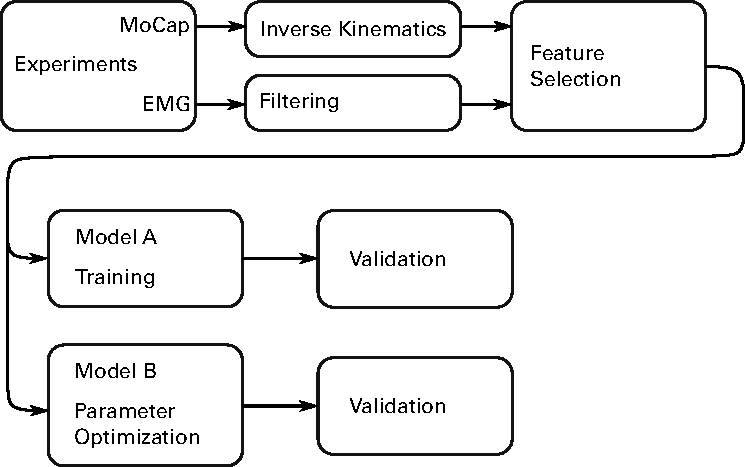
\includegraphics[width=0.8\textwidth]{images/summer_school_study/schematitc.pdf}%
  \caption{Upper Arm Movement Modeling:\\ Schematic workflow of data processing. In experiments, Motion Capture (MoCap) data and EMG signals were recorded. They were processed using inverse kinematics and filtering techniques, respectively. The size of the large datasets was reduced by selecting specific features. Those were used as training inputs for the two models A and B. The trained models were validated using a validation dataset that also originated from experiments.}%
  \label{fig:schematitc}%
\end{figure}%
%
I contributed mainly to the fields of data processing, especially filtering of EMG signals and feature selection, derivation and training of both models, A and B, their validation and the overall programming and visualization of the results. The respective fields are presented more detailed in the following, corresponding sections.

\subsection{Structure of this Chapter}
\Cref{sec:exp_study} gives an overview of the experiments, data processing and feature selection, which resulted in the required datasets. In \cref{sec:study_models}, the two models, A and B, are described. Results including the validation of the models and a discussion are given in \cref{sec:evaluation}. Conclusions follow in \cref{sec:study_conclusion}.

\section{Experimental Study}\label{sec:exp_study}

\begin{figure}%
    \centering%
    \def\svgwidth{5cm}%
    \input{images/summer_school_study/summer_school_study.pdf_tex}%
    \caption{Upper Arm Movement Modeling: \\Experimental setup for the triceps trials. The subject pulls down a rope over a pulley which is connected to a weight with mass $m_w$.
    Angles required for the kinematic formulation are the elbow angle, $\phi_e$, the forearm angle, $\phi_a$, and the angle of the weight, $\phi_w$. The length of the ulna bone is denoted by $\ell_u$.}%
    \label{fig:summer_school_study}%
\end{figure}%

Experiments are required to identify the model parameters for the particular subject. First, the experimental setup is described, then, details on the processing of the measured values are given. Then, the selection of feature points from the experimental data is described.

\subsection{Experimental Trials}

In a series of experiments, eight different actions of flexing and extending the elbow were performed by the subject. Weights of 3 kg and 5 kg were held in the hand during the elbow flexion trials. For the elbow extension trials, a pulley system was installed that redirected the force of the weight such that the downward movement of the forearm acted against the direction of the force. This is shown in \cref{fig:summer_school_study}. A detailed description of the experimental trials can be found in \cite{summerschool2019}.

Time series of position and velocity of the upper arm and the forearm were recorded using a Motion Capture system. It consisted of eight cameras that tracked three markers placed on shoulder, elbow and wrist of the subject. 

The elbow torque $\tau$ was computed as
\begin{equation*}
  \begin{array}{lll}
    \tau = m_w\,g\,\ell_u\,\sin(\phi_w) - m_{a}\,g\,\dfrac{\ell_u}{2}\,\sin(\phi_a),
  \end{array}
\end{equation*}
where $(m_w\,g)$ is the force of the weight, $m_{a}$ is the mass of forearm and hand, $\ell_u$ is the length of the ulna bone and $\phi_a$ and $\phi_w$ are the angles of the forearm and rope, as visualized in \cref{fig:summer_school_study}.

\subsection{Data Processing}
From the captured data, derived quantities of biceps ($B$) and triceps ($T$) muscles were estimated using a geometric model of the upper arm. 
The geometric model is available in the software OpenSim \cite{OpenSim2007} and was customized for the particular subject. The inverse kinematics module of OpenSim was used to estimate the muscle tendon unit lengths, $\ell_{\text{MTU},M}$, contraction velocities, $v_M=\dot{\ell}_M$, and moment arms, $r_{M}$, of the two muscles, $M\in\{B,T\}$.

EMG signals were captured by two electrodes on the skin at the biceps and triceps muscles. For both signals, several preprocessing steps were applied to obtain the inputs for the two models, A and B.

The raw signal was filtered with the same procedure as in \cite{Falisse2016}. First, a fourth-order Butterworth high pass filter with cutoff frequency 30 Hz was applied to reduce non-zero average voltages. Second, the resulting signal was full-wave rectified by taking the absolute value of every measured data point. Third, application of a fourth-order Butterworth low pass filter with 10 Hz cutoff frequency yielded a smoothed signal.
Forth, the resulting filtered EMG signals were normalized to the interval $[0,1]$, such that the value of 1 corresponds to the experimentally determined value of maximum voluntary contraction.

The measured EMG signals on the skin directly correspond to the electric excitation level $u$ in the muscle. Excitation leads to the release of free calcium ions within the sarcomere. Binding of calcium ions to myosin increases the concentration of cross-bridges. This concentration is commonly known as the muscular activation $\alpha$. The muscular activation directly corresponds to the produced force of the muscle \cite{Bayer2017}.

The concentration of free calcium ions is denoted as $\gamma$ and can be computed from the excitation $u$ by the following first order differential equation \cite{Hatze1977}
%
\begin{equation*}
  \begin{array}{lll}
    \dot{\gamma} = m\,(u - \gamma).
  \end{array}
\end{equation*}
%
We used the filtered EMG signal $u$ to obtain values for $\gamma$. \Cref{fig:emg_filtering} shows the raw and filtered EMG signals and the resulting free calcium concentration for a sample of the experimental data.

\begin{figure}%
  \centering%
  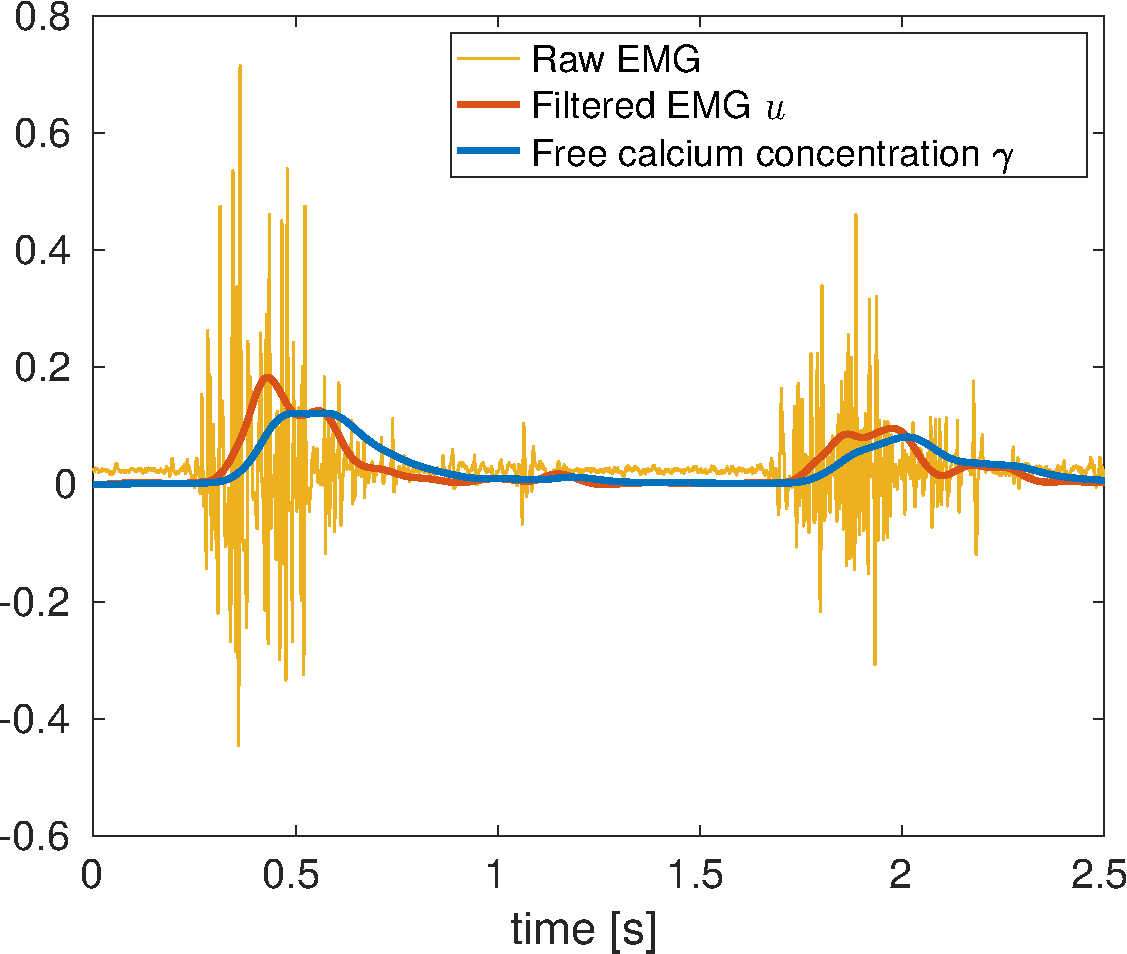
\includegraphics[width=0.8\textwidth]{images/summer_school_study/emg_filtering.pdf}%
  \caption{From raw EMG data of the biceps (yellow) to the filtered signal $u$ (red) and the free calcium concentration $\gamma$ (blue). The data are taken from the beginning of the first elbow flexion experiment. It can be seen that the filtering smooths out the initial signal and removes the constant offset. The free calcium ion concentration follows the filtered EMG with a short delay.}%
  \label{fig:emg_filtering}%
\end{figure}%

The activation of the muscle $\alpha$ does not only depend on the free ion concentration $\gamma$ but also on the current state of muscle contraction. This excitation-contraction coupling has to be described by a dynamic system of ODEs and is included in model B.
Therefore, preprocessing is completed with computing the free calcium concentration $\gamma$ and not the activation $\alpha$.

\subsection{Feature Selection} \label{sec:study_feature_selection}

The eight experimental trials were split into $n_\text{trials}=7$ experiments to be used for model identification and one for validation.
The total number $N$ of captured values in the training experiments was large, such that not all points could be used for training of models A and B.
To reduce the amount of data and, thus, speed up the computation, we selected $n \ll N$ featured values with the assumption that they are representative for the whole data set.
For every experimental trial, we choose the same fixed number $n_\text{per\_trial}$ of data points.
Our selection algorithm identifies $n_\text{per\_trial}$ timesteps, $t_i, i=1, \dots, n$ such that the summed values of the free calcium concentrations $\gamma_B(t_i) + \gamma_T(t_i)$ for biceps and triceps are evenly distributed along the value range.
This leads to $n = n_\text{trials} \cdot n_\text{per\_trial}$ selected data points.

The set of training data $\mathcal{D} = \mathcal{X} \times \mathcal{Y}$ consists of the $n$ selected vectors of the experimental values that are the input to the system of muscles, $\bfx_i \in \mathcal{X}, i=1,\dots, n$, together with the observed output values, $y_i \in \mathcal{Y}, i=1,\dots,n$.
The input vectors contain values for muscle tendon unit lengths, contraction velocities, moment arms and free calcium ion concentrations for biceps and triceps each, $\bfx_i = (\ell_{\text{MTU},B}, \ell_{\text{MTU},T}, v_B, v_T, r_{B}, r_{T}, \gamma_B, \gamma_T)^\top(t_i)$. The output values consist of the elbow torques, $y_i = \tau(t_i)$. This data set, $\mathcal{D}$, serves as training input for both models, A and B.

\section{Models}\label{sec:study_models}

The current section describes the two model approaches that can predict elbow torques from experimental input data. \Cref{sec:data_driven_model} introduces the non-parametric, data driven model A. \Cref{sec:biophysical_model} presents the biophysically based model B. It requires a parameter optimization, which is described in \cref{sec:parameter_optimization}.

\subsection{Data-driven Model A}\label{sec:data_driven_model}

The first modeling approach uses a non-parametric model. Such a model approximates the function $f$ that maps from input to output data points. The function $f$ is learned from the training data set. Regression is used to obtain predictions for new data points. In our case, we use a stochastic model that considers the probability distribution of the model function.

We use the method of \emph{Gaussian Process Regression}. A Gaussian process is a collection of random variables such that the joint distribution of every finite subset of these random variables is multivariate normal (Gaussian).
In our example, each input data point in the space of measured values, $\bfx \in \mathcal{X}$ has an associated random variable $f(\bfx)$ that describes the output of the model for this point.

A Gaussian process, $\mathcal{GP}$, is characterized by a mean function $m(\bfx)$ and a kernel function $k(\bfx,\bfx')$ that models the covariance between any pair $(\bfx, \bfx') \in \mathcal{X} \times \mathcal{X}$ of points. Different choices of kernel functions are possible and can depend on hyperparameters $\bfpsi$. Describing observed values $y$ by a Gaussian process distribution can be expressed as
\begin{equation*}
  \begin{array}{lll}
    f(x) \approx y \sim \mathcal{GP}\big(m(\bfx), k(\bfx,\bfx',\bfpsi)\big).
  \end{array}
\end{equation*}
This representation is non-parametric in the sense that no particular parametric form of the function $y=f(\bfx)$ is assumed whose (biophysical) parameters would be determined. Instead, a generic probabilistic model is constructed using the observed function values at measured inputs $\bfx_i \in \mathcal{X}$.
%More specifically, the conditional distribution $p(y|\bfx)$ considered.

Gaussian Process Regression is based on \emph{Bayesian Inference} to update a prior belief of the model to a posterior model using information contained in observations of the process.
The observed data are the set of measurements $\mathcal{D}$. 

The \emph{prior} distribution $p(\bff\mid\mathcal{X},\bfpsi)$ for the vector of function values $\bff$ is described by the Gaussian process,
\begin{equation*}
  \begin{array}{lll}
    p(\bff\mid\mathcal{X},\bfpsi) = \mathcal{N}(\bff\mid\bfm,\bfK),
  \end{array}
\end{equation*}
with mean values $\bfm = (m(\bfx_i))^\top_{i=1,\dots,n}$ and covariance matrix $\bfK$ with $K_{ij} = k(\bfx_i,\bfx_j,\bfpsi).$

The \emph{likelihood} $p(\bfy\mid f(\bfx), \bftheta)$ describes the probability of an observation $\bfy$ given a particular model $f$. The vector $\bftheta$ denotes additional parameters of the likelihood. 

Using Bayes' rule, the \emph{posterior} distribution $p(\bff\mid\mathcal{D})$ of the function values $\bff$ can be computed from prior and likelihood as
\begin{equation*}
  \begin{array}{lll}
    p(\bff\mid\mathcal{D},\bftheta,\bfpsi) 
      = \dfrac{p(\bfy\mid\bff,\bftheta)\,p(\bff\mid\mathcal{X},\bfpsi)}{p(\mathcal{D}\mid\bftheta,\bfpsi)}.
  \end{array}
\end{equation*}
This results in a measure for the uncertainty of the model $f$ at unobserved points $\bfx_\ast \notin \mathcal{D}$. 

Additionally, the fact that the measured quantities in the experiments are subject to measurement noise can be incorporated into the model.
The assumption 
\begin{equation*}
  \begin{array}{lll}
    y = f(\bfx) + \eps
  \end{array}
\end{equation*}
adds a normally distributed random variable of observational noise $\eps \sim \mathcal{N}(0,\sigma_n^2)$ to the formulation. The noise variance $\theta = \sigma_n^2$ is an additional parameter of the likelihood. 
It is also possible to explicitly model the mean function $m(\bfx)$. By replacing the model $f(\bfx)$ by $g(\bfx) = f(\bfx) + \bfh(\bfx)^\top \bfbeta$, i.e.
\begin{align*}
  %\begin{array}{rlrl}
    y &= f(\bfx) + \bfh(\bfx)^\top \bfbeta + \eps, \quad 
    &\text{ with } f(x) &\sim\mathcal{GP} \big(m(\bfx), k(\bfx,\bfx',\bfpsi)\big),\\[4mm]
    && \eps &\sim \mathcal{N}(0,\sigma_n^2),
  %\end{array}
\end{align*}
we allow for a global trend in the data that is formulated in terms of a vector of explicit basis functions $\bfh(\bfx)$ and corresponding coefficients $\bfbeta$.

The algorithm for Gaussian Process Regression involves estimating the following values from the given data during the training phase. The hyperparameters of the covariance function $\bfpsi$, the noise variance $\bftheta$, and the coefficients of the fixed basis functions $\bfbeta$ are determined by solving an optimization problem. The computation involves matrix inversions and has a computational complexity $\O(n^3)$, i.e. is cubic in the number of data points. For details, the reader is referred to the literature \cite{Rasmussen2005,kuss2006gaussian}.

In our study, training of the Gaussian Process of model A was performed using the ready to use implementation provided by MATLAB.
We parametrized the covariance by a squared exponential kernel and used constant basis functions, $\bfh(x) = 1$. We enabled observational noise, its variance $\bftheta = \sigma_n^2$ was found by optimization during training of the model.

%$p(\bff^\ast | \mathcal{D},\mathcal{X}^\ast)$
\subsection{Biophysical Model B}\label{sec:biophysical_model}

Extension of the elbow is governed by the triceps brachii muscle.
During elbow flexion, three muscles are involved: biceps brachii, brachialis and brachioradialis. For simplicity, only biceps brachii, which contributes most of the moment, is explicitly considered in the current study. The effects of the other two muscle are contained in the biceps brachii model in a lumped manner.

Thus, the biophysical model consists of two Hill-type muscle models, for biceps and triceps, respectively. The muscle models are arranged around a hinge joint for the elbow angle. The muscle forces contribute to the torque at the elbow over their respective moment arms.

Hill-type models describe the macroscopic, dynamic mechanical behavior of an entire muscle along a one-dimensional line of action.
The behavior is formulated by phenomenological, mathematical functions that have to be parametrized to fit experimental observations.

%Such models are often used to compute muscle forces in simulations of various movements, e.g. \cite{Siebert2003}, \cite{Kistemaker2006}.
Multiple variants of Hill-type models exist that use various configurations of mechanical elements to consider different properties and functionalities of the muscle. The original model was proposed in \cite{Hill1938}. It contains a contractile element (CE) and two elastic elements, arranged in series and in parallel to the CE.
The authors of \cite{Siebert2008} compare two different approaches using these three elements. The effect of tension in eccentric contractions is added to the Hill-type model by \cite{Till2008}. The authors of \cite{Gunther2007} add a forth, damping element to account for high-frequency damping of the muscle tissue. In \cite{Morl2012}, electromechanical delay is investigated with and without the additional damping element. 

\begin{figure}%
  \centering%
  \def\svgwidth{0.5\textwidth}
  \input{images/summer_school_study/hilltype.pdf_tex}%
  \caption{Mechanical structure of the Hill-type muscle model. The force generating contractile element (CE) is parallel-connected to the parallel elastic element (PEE) and connected in series to a second parallel-connected structure consisting of the serial elastic element (SEE) and the serial damping element (SDE). The length $l_\text{MTU}$ of the whole muscle tendon unit is composed of the common length $l_\text{CE}$ of CE and PEE and the common length $l_\text{SEE}$ of SEE and SDE. The variable $l_\text{CE}$ is an internal state of the model.}
  \label{fig:hilltype}%
\end{figure}%

\newcommand{\CE}{\text{CE}}
\newcommand{\MTU}{\text{MTU}}

We employ the four-element Hill-type muscle model that is described by \cite{Hilltype2014}. Its structure is visualized in \cref{fig:hilltype}. It consists of four components: the contractile element (CE), the parallel elastic element (PEE), the serial elastic element (SEE), and the serial damping element (SDE). Inputs to the model are the muscular activation $\alpha(t)$, the length $l_\MTU(t)$ and the contraction velocity $\dot{l}_\MTU(t)$ of the muscle tendon unit (MTU).
The output of the model is the muscle force $f_\text{MTU}(t)$. The model contains one internal state variable, the length $l_\text{CE}(t)$ of the CE. The muscle dynamics determine this internal length and its time derivative, the contraction velocity $\dot{l}_\text{CE}(t)$ of the CE.

The resulting force of the MTU is given as sum of the forces of the respective parallel elements as visualized in \cref{fig:hilltype}:
\begin{equation}\label{eq:hill_type0}
  \begin{array}{lll}
    F_\MTU = F_\CE(l_\CE, \dot{l}_\CE, \alpha) + F_\text{PEE}(l_\CE) = F_\text{SEE}(l_\CE,l_\MTU) + F_\text{SDE}(l_\CE,\dot{l}_\CE,\dot{l}_\MTU,\alpha).
  \end{array}
\end{equation}
The force terms of the four elements, $F_\CE, F_\text{PEE}, F_\text{SEE}$ and $F_\text{SDE}$ are described by analytical functions that use a total of 19 parameters. A description of the detailed equations and parameters can be found in \cite{Hilltype2014}. In the following, an overview over the formulation is given with a focus on the piecewise formulated terms that contribute to the overall muscle model. In the following formulations, underlined variables designate constant parameters that either have to be specified or follow from other given parameters.

The muscle output force $F_\text{MTU}$ is computed by the second identity of \cref{eq:hill_type0}, i.e., from the forces $F_\text{SEE}$ and $F_\text{SDE}$. The force $F_\text{SEE}$ acting in the SEE is formulated as a continuous piecewise function with a constant zero, an exponential and a linear branch:
\begin{equation*}
  \begin{array}{lll}
    F_\text{SEE}(\ell_\CE,\ell_\MTU) = \begin{cases}
      0, & \ell_\text{SEE} < \underline{l_{\text{SEE},0}}\\[2mm]
      \underline{K_\text{SEE,nl}}(\ell_\text{SEE} - \underline{\ell_\text{SEE,0}})^{\underline{\nu_\text{SEE}}}, & \ell_\text{SEE} < \underline{\ell_\text{SEE,nll}}\\[2mm]
    \underline{\Delta F_\text{SEE,0}} + \underline{K_\text{SEE,l}}(\ell_\text{SEE} - \underline{\ell_\text{SEE,nll}}), & 
    \ell_\text{SEE} \geq \underline{\ell_\text{SEE,nll}}
    \end{cases}, \quad \text{with } \ell_\text{SEE} = \ell_\MTU - \ell_\CE.
  \end{array}
\end{equation*}

The damping force $F_\text{SDE}$ in the SDE is proportional to the lengthening velocity ${\dot{\ell}_\text{SEE} = \dot{\ell}_\MTU - \dot{\ell}_\CE}$ of this element. It is given by
\begin{equation}\label{eq:sde_force}
  \begin{array}{lll}
    F_\text{SDE}(l_\CE,\dot{l}_\CE,\dot{l}_\MTU,\alpha) \\ \qquad = \underline{D_\text{SDE,max}}\left( (1-\underline{R_\text{SDE}}) \dfrac{F_\text{PEE}(\ell_\CE)+F_\text{CE}(\ell_\CE, \dot{\ell}_\CE, \alpha)}{\underline{F_\text{max}} + \underline{R_\text{SDE}}} \right) (\dot{\ell}_\MTU - \dot{\ell}_\CE).
  \end{array}
\end{equation}
The amount of damping is dependent on the force $F_\MTU$ of the MTU which appears in the nominator of the fraction in \cref{eq:sde_force} as the sum of the forces $F_\text{PEE}$ and $F_\CE$. Formulas for these two forces are given in the following.

The force $F_\text{PEE}$ of the PEE is formulated piecewise as a shifted and cut off polynomial function:
\begin{equation}\label{eq:fpee}
  \begin{array}{lll}
    F_\text{PEE}(\ell_\CE) = \begin{cases}
      0, & \ell_\CE < \underline{\ell_{\text{PEE},0}}\\[4mm]
    \underline{K_\text{PEE}}(l_\CE - \underline{l_{\text{PEE},0}})^{\underline{\nu_\text{PEE}}},& \ell_\CE \geq \underline{\ell_{\text{PEE},0}}
    \end{cases}.
  \end{array}
\end{equation}

The force $F_\CE$ of the CE is the active force produced by the muscle and is given by:
\begin{equation}\label{eq:fce}
  \begin{array}{lll}
    F_\CE(l_\CE, \dot{l}_\CE, \alpha) 
    = \underline{F_\text{max}} \left(
    \dfrac{\alpha\,F_\text{isom}(\ell_\CE) + A_\text{rel}(\dot{\ell}_\CE,\ell_\CE,\alpha)}
    {1 - 
    \frac{\dot{\ell}_\CE}
    {B_\text{rel}(\dot{\ell}_\CE,\ell_\CE,\alpha)\,\ell_{\CE,\text{opt}}}}\right)
    - A_\text{rel}(\dot{\ell}_\CE,\ell_\CE,\alpha).
  \end{array}
\end{equation}
It can be seen that the active force depends on the activation level $\alpha$. 
The formulation of $F_\CE$ contains the two main characteristic curves for muscle forces, the force-length relation and the force-velocity relation.

The force-length relation is modeled by the function $F_\text{isom}(\ell_\CE)$ of isometric force, which describes the relative force for the condition $\dot{\ell}_\CE = 0$. This function is formulated piecewise for CE lengths $\ell_\CE$ smaller and larger than an optimal length $\ell_\text{CE,opt}$. 

The force-velocity relation follows from the auxiliary functions $A_\text{rel}(\dot{\ell}_\CE,\ell_\CE,\alpha)$ and $B_\text{rel}(\dot{\ell}_\CE,\ell_\CE,\alpha)$. These functions have different forms for concentric ($\dot{\ell}_\CE < 0$) and eccentric ($\dot{\ell}_\CE \geq 0$) conditions as well as for the two ranges of CE  length, $\ell_\CE < \ell_\text{CE,opt}$ and $\ell_\CE \geq \ell_\text{CE,opt}$.

\begin{figure}%
  \centering%
  \begin{subfigure}[t]{0.9\textwidth}%
    \centering%
    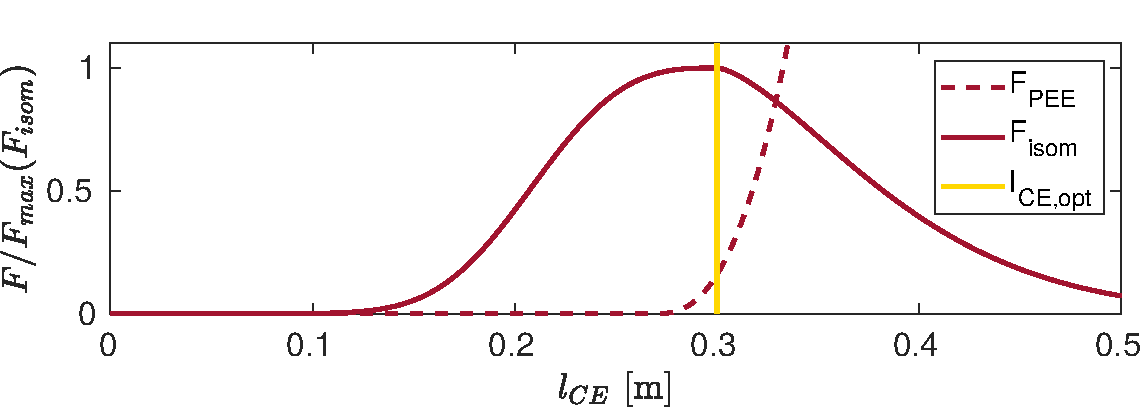
\includegraphics[width=\textwidth]{images/summer_school_study/force_curves_generic_length.pdf}%
    \caption{Force-length curves of the PEE (dashed red line) and isometric force $F_\text{isom}$ (solid red line) for an isometric condition ($\dot{l}_\CE=0$), normalized to the maximum isometric force. The optimal length $l_\text{CE,opt}$ of the CE is shown as yellow vertical line. The force $F_\text{PEE}(l_\CE)$ of the PEE is zero for $l_\CE < 0.9\,l_\text{CE,opt}$. The isometric contraction force $F_\text{isom}$ is formulated piecewise by two branches separated by $l_\text{CE,opt}$.}%
    \label{fig:force_curves_generic_length}%
  \end{subfigure}\\[6mm]
  \begin{subfigure}[t]{0.9\textwidth}%
    \centering%
    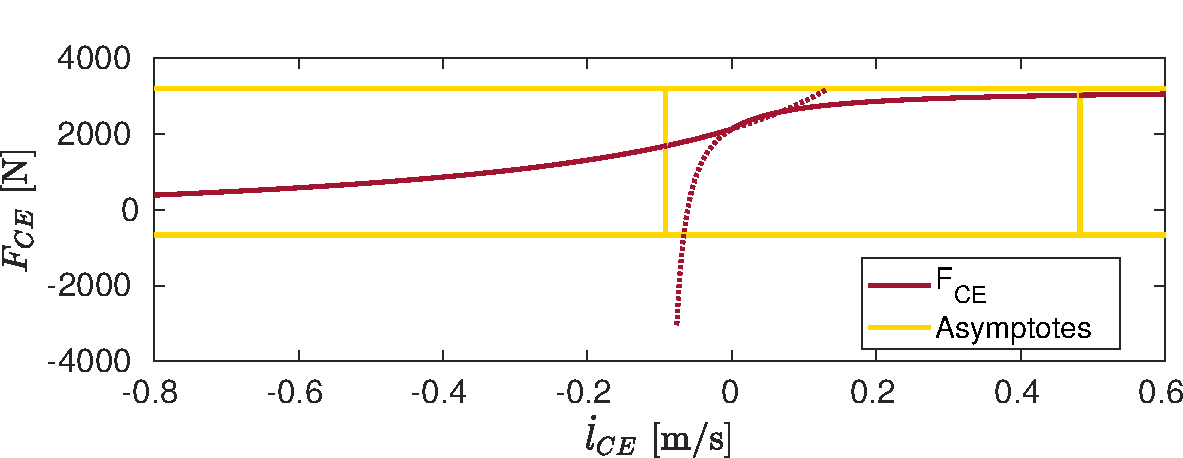
\includegraphics[width=\textwidth]{images/summer_school_study/force_curves_generic_velocity.pdf}%
    \caption{Force-velocity curve $F_\CE(\dot{l}_\CE)$ of the CE at optimal length $l_\CE=l_{\CE,\text{opt}}$, and for activation level $\alpha=0.5$. The function (red solid line) is formulated piecewise, graphs of the base functions of the two branches continue as red dotted lines. Their limits and singularities are visualized by the yellow horizontal and vertical asymptotes.}%
    \label{fig:force_curves_generic_velocity}%
  \end{subfigure}%
  \caption{Force-length and force-velocity relations for the muscle model with generic parameters taken from literature \cite{Hilltype2014}.}%
  \label{fig:force_curves_generic}%
\end{figure}%

\Cref{fig:force_curves_generic} visualizes the two main characteristic curves of the model. 
\Cref{fig:force_curves_generic_length} shows how the generated force depends on the length of the CE. 
The active force $F_\CE$, given by \cref{eq:fce}, is visualized by the solid red line. It has its maximum at the optimal length $l_\text{CE,opt}$ of the CE. This can be explained by the overlap of actin and myosin filaments in the sarcomere. The overlap is lower when the actin filaments are pulled apart or pushed together. A higher overlap leads to a higher force output.

The dashed line in \cref{fig:force_curves_generic_length} represents the passive force $F_\text{PEE}$ of the elastic muscular tissue, formulated in \cref{eq:fpee}. The passive force is essentially generated by the titin proteins in the sarcomere. Only starting from a certain length, the structure exerts reaction forces against lengthening forces to avoid overstretching of the muscle.

\cref{fig:force_curves_generic_velocity} shows the force-velocity relation of the Hill-type model. The curve of $F_\CE(\dot{l}_\CE)$ is composed of two branches: 
The concentric branch for shortening contraction with $\dot{l}_\CE \leq 0$ and the eccentric branch for lengthening contraction with $\dot{l}_\CE > 0$. It can be seen that the generated force increases monotonically over the lengthening velocity. It approaches a limit for maximum positive and negative velocity. These limits can be adjusted by parameters of the model and are exemplary for how the shape of the curves of a Hill-type model can be parametrized.

In addition to the resulting muscle force $F_\MTU$, a formulation for the internal state variable $\ell_\CE$ is required.
The second identity of \eqref{eq:hill_type0} can be solved for the lengthening velocity $\dot{\ell}_\CE$ of the CE to get an evolution equation for the length $\ell_\CE$ of the CE. The derivation and the resulting formula can be found in \cite{Hilltype2014}.

To describe the activation dynamics, i.e., the evolution of the muscle activation ${\alpha \in [0,1]}$, the model of Hatze et al. \cite{Hatze1977} is used.
The activation is computed depending on the free calcium ion concentration $\gamma$ and the length $\ell_\CE$ of the CE by
\begin{equation*}
  \begin{array}{lll}
    \alpha(\ell_\CE,\gamma) = \dfrac{\underline{a_0} + \big(\rho(\ell_\CE)\,\gamma\big)^3}
    {1 + \big(\rho(\ell_\CE)\,\gamma\big)^3}.
  \end{array}
\end{equation*}
The function $\rho$ is given by
\begin{equation*}
  \begin{array}{lll}
    \rho(\ell_\CE) = \underline{c}\,\underline{\eta}\,\dfrac{(\underline{k}-1)\,\ell_\CE}{(\underline{k} - \ell_\CE/\ell_\text{CE,opt})\,l_\text{CE,opt}}.
  \end{array}
\end{equation*}
All used parameter values for the activation dynamics can be found in \cite{Bayer2017}.

In summary, we get the following coupled system of differential-algebraic equations, where $f_\CE$ and $f_\alpha$ denote the respective formulas:
\begin{align}
  F_\MTU &= F_\MTU(\ell_\MTU,l_\CE,\dot{l}_\CE,\alpha),      \label{eq:hill_type1} \\[4mm]
  \dot{l}_\CE &= f_\CE(l_\CE,\ell_\MTU,\dot{l}_\MTU,\alpha), \label{eq:hill_type2}\\[4mm]
  \alpha &= f_\alpha(\gamma, l_\CE).                      \label{eq:hill_type3}
\end{align}

To compute the joint torque in a system of an agonist and antagonist muscle pair, two instances of the presented Hill-type muscle model can be used. In our study considering the upper arm, the torque $\tau$ at the elbow is computed by multiplying the predicted forces $F_{\MTU,B}$ and $F_{\MTU,T}$ of biceps and triceps with the corresponding moment arms $\hat{r}_B$ and $\hat{r}_T$:
\begin{equation}\label{eq:muscle_torque}
  \begin{array}{lll}
    \tau = F_{\MTU,B}(l_{\MTU,B},\dot{l}_{\MTU,B},\alpha_B) \cdot \hat{r}_B - F_{\MTU,T}(l_{\MTU,T},\dot{l}_{\MTU,T},\alpha_T) \cdot \hat{r}_T.
  \end{array}
\end{equation}

\subsection{Parameter Identification for Model B}\label{sec:parameter_optimization}
%
The process of model identification finds the parameters that make the model B predict correct values for the specific subject, i.e., minimizes the error in the predicted outcome for the training data set.

The following minimization is performed:
\begin{align}
  &&\min\limits_{\substack{\bftheta_M,l_{\CE,M}(t), \\\forall M \in \{B,T\}, \,\forall t \in \mathcal{T}}} &\sum\limits_{t\in \mathcal{T}}|\tau(t) - \hat{\tau}(t)|^2
   \label{eq:opt_1}\\[4mm]
  &&\text{s.t. }\forall t \in \mathcal{T}:\quad &\tau(t) = F_{\MTU,B}(t,l_{\CE,B},\bftheta_B) \cdot \hat{r}_B(t) \notag\\
      &&&\qquad\quad- F_{\MTU,T}(t,l_{\CE,T},\bftheta_T) \cdot \hat{r}_T(t),                 \label{eq:opt_2}\\[4mm]
  &&& \dot{l}_{\CE,M}(t) = \dot{\hat{l}}_{\MTU,M}(t),\quad M \in \{B,T\},      \label{eq:opt_3}\\[4mm]
  &&& \bftheta_B, \bftheta_T \in \Theta,                                       \label{eq:opt_4}\\[4mm]
  &&& l_{\CE,M}(t) \in [0,l_{\MTU,M}(t)],\quad M \in \{B,T\}.                  \label{eq:opt_5}
\end{align}

The optimization variables are the parameters $\bftheta_B$ and $\bftheta_T$ for the biceps and triceps Hill-type models and the lengths $l_{\CE,B}(t)$ and $l_{\CE,T}(t)$ of the contractile elements for both models at every point in time. The variables designated as $\hat{\square}$ are the measured quantities from the training experiments. The objective function given in \cref{eq:opt_1} penalizes the difference between computed torque $\tau$ and measured torque $\hat{\tau}$ at every timestep $t \in \mathcal{T}$ of the training data. 

\Cref{eq:opt_2} computes the torque values and follows from \cref{eq:muscle_torque} of the muscle model. For every point in time, the predicted forces $F_{\MTU,B}$ and $F_{\MTU,T}$ are multiplied with the measured moment arms $\hat{r}_B$ and $\hat{r}_T$.

In \cref{eq:opt_3}, the contraction velocities are constrained to the measured values. Because the lengthening velocity $\dot{l}_\CE$ of the CE is an internal quantity and, thus, cannot be observed in experiments, we assume it to be equal to the lengthening velocity of the whole muscle: $\dot{l}_\CE \approx \dot{l}_{\MTU} = \dot{l}_\text{CE} + \dot{l}_\text{SEE}$. This requires the assumption $\dot{l}_{\text{SEE}} \approx 0$ which can be justified given the low dynamic nature of the experiments.

By \cref{eq:opt_4}, we bound each of the parameters $\bftheta_B$ and $\bftheta_T$ to a range between half and twice the generic value from literature.
The lengths of the CEs are constrained by \cref{eq:opt_5} to be positive and smaller than the length of the MTU.

All optimization variables are normalized to improve the numerical conditioning of the optimization problem. 
The parameters $\bftheta_B$ and $\bftheta_T$ are normalized with respect to generic values from literature that were taken from \cite{Gunther2007, Morl2012, Hilltype2014}. The initial values are set to one, which corresponds to the generic literature values.
The internal states $l_{\CE,B}$ and $l_{\CE,T}$, are normalized with respect to the measured MTU lengths $\hat{l}_{\MTU,B}$ and $\hat{l}_{\MTU,T}$ and initialized with zero.

%For training of model B, the optimization problem for the parameters needed to be solved. 
We implemented the Hill-type models and the constraints in MATLAB and used the nonlinear programming implementation, \code{fmincon}, to minimize the given bounded and nonlinear constrained, multivariable function.
In our study, the total number of optimization variables is computed by $2\cdot 19 + 2n = 598$, as each of the parameter vectors $\bftheta_B,\bftheta_T$ had 19 entries. 

\section{Results and Discussion}\label{sec:evaluation}

In the following, results of connecting the two model formulations, A and B, to the experimental data are presented.
At first, \cref{sec:res_feature_selection} gives details on the preprocessed data. The training phase is described in \cref{sec:res_training}. Applying the trained models to the validation data is done in \cref{sec:res_validation}. Then, \cref{sec:res_simplified_a} tests a simplified version for model A. Then, \cref{ref:res_insights_b} shows some insights into the optimized parameter values for model B.

\subsection{Feature Selection}\label{sec:res_feature_selection}
% intro
The experimental data is split into a training and a validation dataset. \Cref{fig:selected_points} shows the processed data of the training data set. In total, we captured $N=\num{34934}$ data points for the seven experimental trials. Out of these, we select $n_\text{per\_trial}=\num{40}$ feature points in every trial, leading to a total of $n=n_\text{per\_trial}\cdot n_\text{trials}=\num{280}$ points. The selected points are visualized by crosses in the top plot of \cref{fig:selected_points}. It can be seen that the algorithm described in \cref{sec:study_feature_selection} distributes the feature points equally along the $\gamma$ axis.

\begin{figure}%
  \centering%
  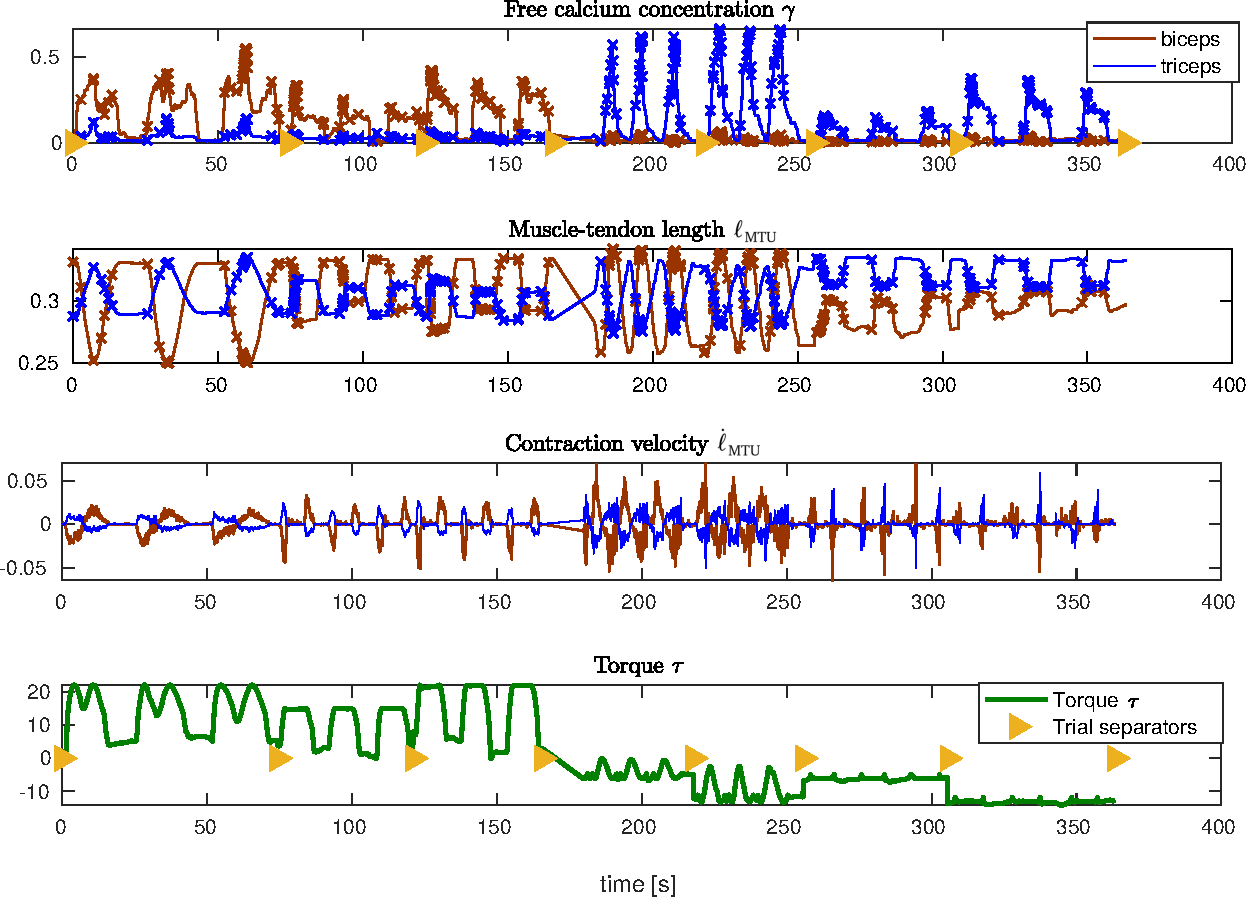
\includegraphics[width=\textwidth]{images/summer_school_study/selected_points.pdf}%
  \caption{Processed experimental values over time that were used for training of both models. The concatenated data of seven trials are shown, which yield an end time of $\SI{363.32}{s}$. The individual trials are separated by the yellow triangles on the $x$-axis. The three upper plots show the values of $\gamma, \ell_\MTU$ and $\dot{l}_\MTU$ for both biceps (brown) and triceps (blue), the bottom plot shows the elbow torque $\tau$. The selected feature points are visualized as crosses in the two top plots. In the upper-most plot, it can be seen that the first three trials, which correspond to elbow flexion, mainly activated the biceps muscle, whereas in the last four trials, corresponding to elbow extension, the triceps is more active.
}%
  \label{fig:selected_points}%
\end{figure}%

\subsection{Training of the Models}\label{sec:res_training}
%
Training of model A consists of estimating the hyperparameters for the Gaussian Process Regression model from the training data.

For model B, the optimization problem for the biophysical parameters is solved. The resulting parameter values and their relation to the initial values are summarized in \cref{tab:model_b_parameters}. It can be seen that none of the final parameter values is limited by the constraints, which would be $\SI{-50}{\percent}$ and +\SI{100}\percent. However, it was observed that including the constraints helps the optimizer to stay in the valid range of meaningful model parameters and, thus, reach the optimum faster.

\begin{table}[t] 
  \centering
  %\begin{scriptsize}
  
    \begin{tabular}{@{}llllll@{}}
%\hline
 %| param              | biceps   |            | triceps  |            %|
 %| ------------------ | -------- | ---------- | -------- | ---------- %|
 %| CE_F_max           | +11.03 % | 4729.97    | -49.04 % | 2171.04    |
 %| CE_l_CEopt         | +31.72 % | 0.40       | -25.36 % | 0.22       |
 %| CE_DeltaW_limb_des | +10.86 % | 0.39       | +10.86 % | 0.39       |
 %| CE_DeltaW_limb_asc | +91.61 % | 0.67       | +5.05 %  | 0.37       |
 %| CE_v_CElimb_des    | +10.86 % | 1.66       | +10.86 % | 1.66       %|
 %| CE_v_CElimb_asc    | -46.39 % | 1.61       | +95.87 % | 5.88       |
 %| CE_A_rel0          | +14.03 % | 0.29       | -20.34 % | 0.20       |
 %| CE_B_rel0          | +77.51 % | 3.99       | +41.38 % | 3.18       |
 %| CE_S_eccentric     | -4.12 %  | 1.92       | +22.92 % | 2.46       |
 %| CE_F_eccentric     | -30.94 % | 1.04       | +36.79 % | 2.05       |
 %| PEE_L_PEE0         | +10.86 % | 1.00       | +10.86 % | 1.00       |
 %| PEE_l_PEE0         | +10.86 % | 0.30       | +10.86 % | 0.30       |
 %| PEE_v_PEE          | +10.86 % | 2.77       | +10.86 % | 2.77       |
 %| PEE_F_PEE          | +10.86 % | 2.22       | +10.86 % | 2.22       |
 %| PEE_K_PEE          | +10.86 % | 1410470.38 | +10.86 % | 1410470.38 |
 %| SDE_D_SE           | +10.86 % | 0.33       | +10.86 % | 0.33       |
 %| SDE_R_SE           | +8.63 %  | 0.01       | -10.99 % | 0.01       |
 %| SDE_d_SEmax        | +8.41 %  | 513.16     | -10.64 % | 422.98     |
 %| SEE_l_SEE0         | -24.95 % | 0.13       | -10.28 % | 0.15       |
 %| SEE_DeltaU_SEEnll  | +59.16 % | 0.07       | +23.58 % | 0.05       |
 %| SEE_DeltaU_SEEl    | +63.34 % | 0.03       | +19.02 % | 0.02       |
 %| SEE_DeltaF_SEE0    | -42.40 % | 327.16     | +64.75 % | 935.78     |
 
% contractile element (CE)
%===========================
%  CE_F_max                         % F_max in [N] for Extensor (Kistemaker et al., 2006)
%  CE_l_CEopt                       % optimal length of CE in [m] for Extensor (Kistemaker et al., 2006)
%* CE_DeltaW_limb_des = 0.35;       % width of normalized bell curve in descending branch (Moerl et al., 2012)
%* CE_DeltaW_limb_asc = 0.35;       % width of normalized bell curve in ascending branch (Moerl et al., 2012)
%* CE_v_CElimb_des = 1.5;           % exponent for descending branch (Moerl et al., 2012)
%  CE_v_CElimb_asc = 3.0;           % exponent for ascending branch (Moerl et al., 2012)
%* CE_A_rel0 = 0.25;                % parameter for contraction dynamics: maximum value of A_rel (Guenther, 1997, S. 82)
%* CE_B_rel0 = 2.25;                % parameter for contraction dynmacis: maximum value of B_rel (Guenther, 1997, S. 82)
%  eccentric force-velocity relation:
%* CE_S_eccentric  = 2;             % relation between F(v) slopes at v_CE=0 (van Soest & Bobbert, 1993)
%  CE_F_eccentric  = 1.5;           % factor by which the force can exceed F_isom for large eccentric velocities (van Soest & Bobbert, 1993)

% paralel elastic element (PEE)
%===============================
%  PEE_L_PEE0   = 0.9;                               % rest length of PEE normalized to optimal lenght of CE (Guenther et al., 2007)
%  PEE_v_PEE    = 2.5;                               % exponent of F_PEE (Moerl et al., 2012)
%  PEE_F_PEE    = 2.0;                               % force of PEE if l_CE is stretched to deltaWlimb_des (Moerl et al., 2012)

% serial damping element (SDE)
%=============================
%* SDE_D_SE    = 0.3;               % xxx dimensionless factor to scale d_SEmax (Moerl et al., 2012)
%* SDE_R_SE    = 0.01;              % minimum value of d_SE normalised to d_SEmax (Moerl et al., 2012)
%  SDE_d_SEmax = SDE_D_SE*(CE_F_max*CE_A_rel0)/(CE_l_CEopt*CE_B_rel0);
                                    % maximum value in d_SE in [Ns/m] (Moerl et al., 2012)

% serial elastic element (SEE)
% ============================
%  SEE_l_SEE0        = 0.172;       % rest length of SEE in [m] (Kistemaker et al., 2006)
%  SEE_DeltaF_SEE0   = 568;         % both force at the transition and force increase in the linear part in [N] (~ 40% of the maximal isometric muscle force)
%  SEE_DeltaU_SEEnll = 0.0425;      % relativ stretch at non-linear linear transition (Moerl et al., 2012)
%* SEE_DeltaU_SEEl   = 0.017;       % relativ additional stretch in the linear part providing a force increase of deltaF_SEE0 (Moerl, 2012)
% 
     \toprule
    \textbf{CE} 
      & $F_{\mathrm{max}}\,[\mathrm{N}]$
      & $l_{\mathrm{CE},opt}\,[\mathrm{m}]$ 
      & $\Delta W_{d} \,[\;]$ 
      & $\Delta W_{a} \,[\;]$ 
      & $\nu_{\mathrm{CE},d} \,[\;]$ \\  \midrule
    Generic & $4260$ & $0.3$ & $0.35$ & $0.35$ & $1.5$  \\ %\hline
    Biceps  & $+\SI{11.0}{\percent}$ & $+\SI{31.7}{\percent}$ & $+\SI{10.9}{\percent}$ & $+\SI{91.6}{\percent}$ & $+\SI{10.9}{\percent}$  \\ %\hline
    Triceps & $-\SI{49.0}{\percent}$ & $-\SI{25.4}{\percent}$ & $+\SI{10.9}{\percent}$ & $+\SI{5.1}{\percent}$ & $+\SI{10.9}{\percent}$  \\ %\hline 
    \addlinespace[2ex]
    \textbf{CE} 
      &  $\nu_{\mathrm{CE},a} \,[\;]$ 
      & $A_\text{rel,0} \,[\;]$  
      & $B_\text{rel,0} \,[\;]$ 
      & $S_\text{ecc} \,[\;]$ 
      & $F_\text{ecc} \,[\;]$\\  \hline
    Generic & $3.0$ & $0.25$ & $2.25$ & $2$ & $1.5$ \\ %\hline
    Biceps & $-\SI{46.4}{\percent}$ & $+\SI{14.0}{\percent}$ & $+\SI{77.5}{\percent}$ & $-\SI{4.1}{\percent}$ & $-\SI{30.1}{\percent}$ \\ %\hline
    Triceps &  $+\SI{95.9}{\percent}$ & $-\SI{20.3}{\percent}$ & $+\SI{41.4}{\percent}$ & $+\SI{22.3}{\percent}$ & $+\SI{36.8}{\percent}$ \\ %\hline
    \addlinespace[2ex]
    \textbf{PEE} 
      & $L_{\mathrm{PEE},0} \,[\;]$ 
      & $\nu_{\mathrm{PEE}} \,[\;]$ 
      & $F_{\mathrm{PEE}} \,[\;]$
      \\ \hline
    Generic & $0.9$ & $2.5$ & $2.0$  \\ %\hline
    Biceps & $+\SI{10.9}{\percent}$ & $+\SI{10.9}{\percent}$ & $+\SI{10.9}{\percent}$  \\ %\hline
    Triceps & $+\SI{10.9}{\percent}$ & $+\SI{10.9}{\percent}$ & $+\SI{10.9}{\percent}$  \\ %\hline
    \addlinespace[2ex]
    \textbf{SDE} 
      & $D_{\mathrm{SDE}} \,[\;]$ 
      & $R_{\mathrm{SDE}} \,[\;]$ 
      \\ \midrule
    Generic & $0.3$ & $0.01$    \\ %\hline
    Biceps & $+\SI{10.9}{\percent}$ & $+\SI{8.6}{\percent}$   \\ %\hline
    Triceps & $+\SI{10.9}{\percent}$ & $-\SI{11.0}{\percent}$  \\ %\hline
    \addlinespace[2ex]
    \textbf{SEE} 
      & $l_{\mathrm{SEE},0}\,[\mathrm{m}]$ 
      & $\Delta F_{\mathrm{SEE},0} \,[\;]$  
      & $\Delta U_\text{l} \,[\;]$  
      & $\Delta U_\text{nll}\,[\;]$
      \\ \hline
    Generic & $0.172$ & $0.0425$ & $0.017$ & $568$ \\ %\hline
    Biceps & $-\SI{25.0}{\percent}$ & $-\SI{42.4}{\percent}$ & $+\SI{63.3}{\percent}$ & $+\SI{59.2}{\percent}$ \\ %\hline
    Triceps & $-\SI{10.3}{\percent}$ & $+\SI{64.75}{\percent}$ & $+\SI{19.0}{\percent}$ & $+\SI{23.6}{\percent}$ \\ %\hline
    \bottomrule
  \end{tabular}

  \caption{Hill-type muscle model parameters of the four elements: CE, PEE, SDE and SEE, initial values given in literature and relative changes of the optimized values. Further explanations of the parameters and references to literature containing their initial values are given in \cite{Hilltype2014}.}
  \label{tab:model_b_parameters}
  %\end{scriptsize}
\end{table}

After training of the models A and B using the selected points of the training dataset, both models were tested by a \emph{resubstitution prediction}, i.e., predicting output from the training input data. The results are shown in \cref{fig:measured_optimized_torque_A} for model A and \cref{fig:measured_optimized_torque_B} for model B. As this evaluation only uses the subset of selected experimental values, the data points have no natural ordering. They were sorted for better visibility.

It can be seen that, for both models, the predicted values are a good fit to the measured values. For model A, the predicted 95\% confidence interval includes the actually measured values almost everywhere. For model B, the predicted values show a higher variance, especially for high torque values.

\begin{figure}%
  \centering%
  \begin{subfigure}[t]{0.48\textwidth}%
    \centering%
    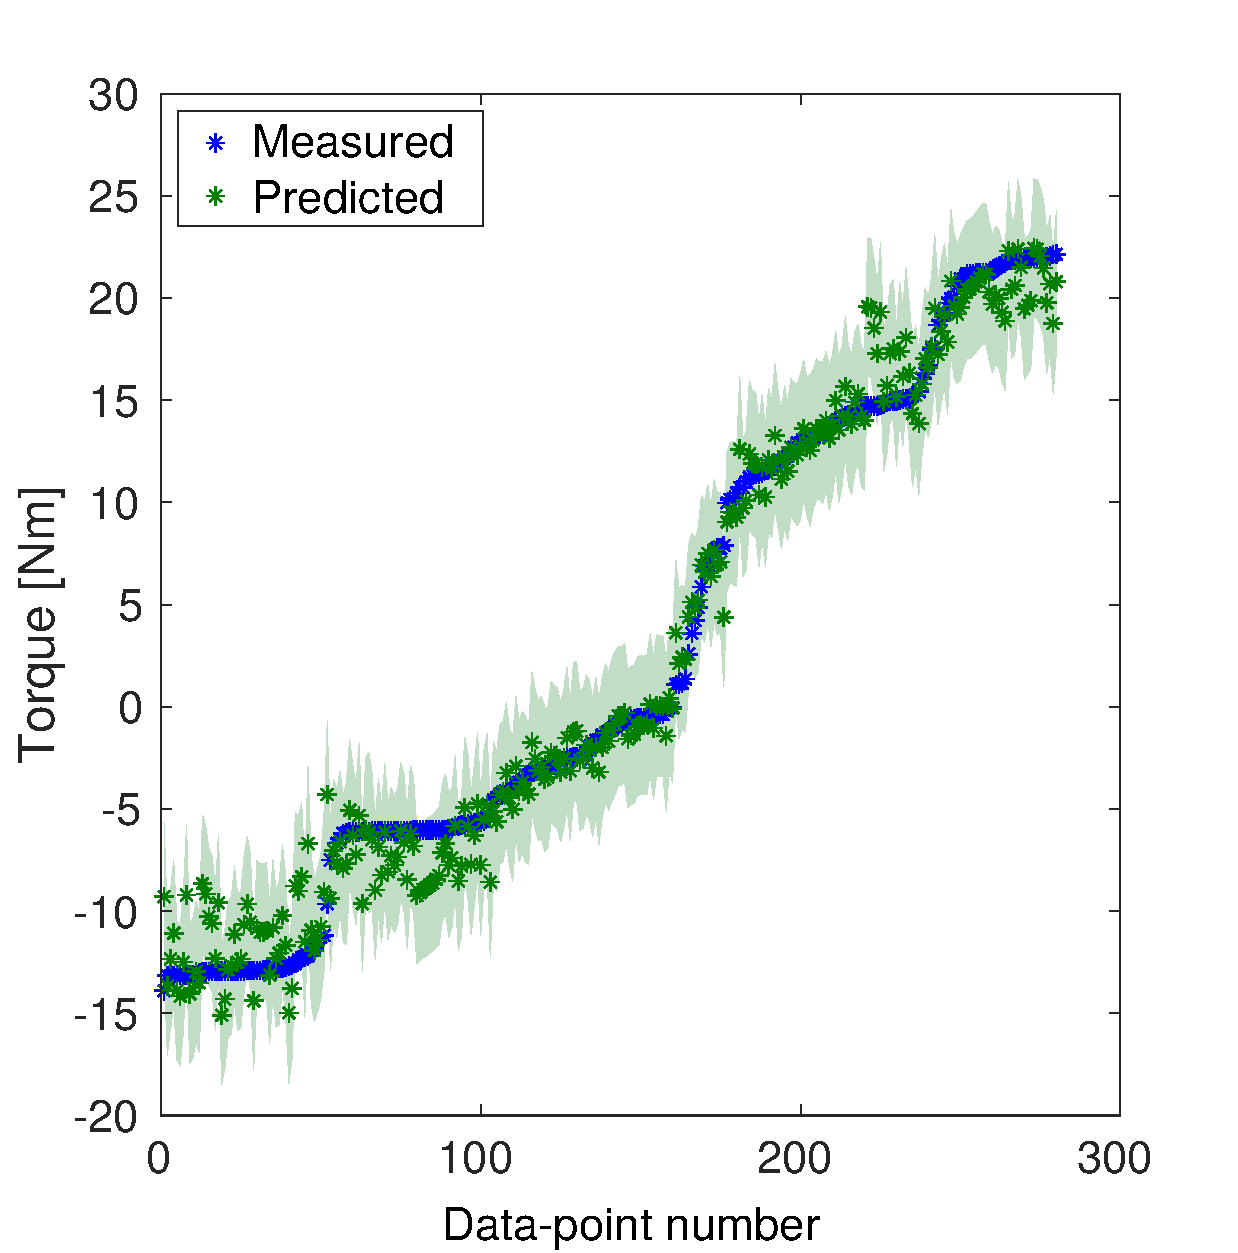
\includegraphics[width=\textwidth]{images/summer_school_study/measured_optimized_torque_A.pdf}%
    \caption{Measured values (blue) and values predicted by model A (dark green), with 95\% confidence interval (light green).}%
    \label{fig:measured_optimized_torque_A}%
  \end{subfigure}%
  \quad
  \begin{subfigure}[t]{0.48\textwidth}%
    \centering%
    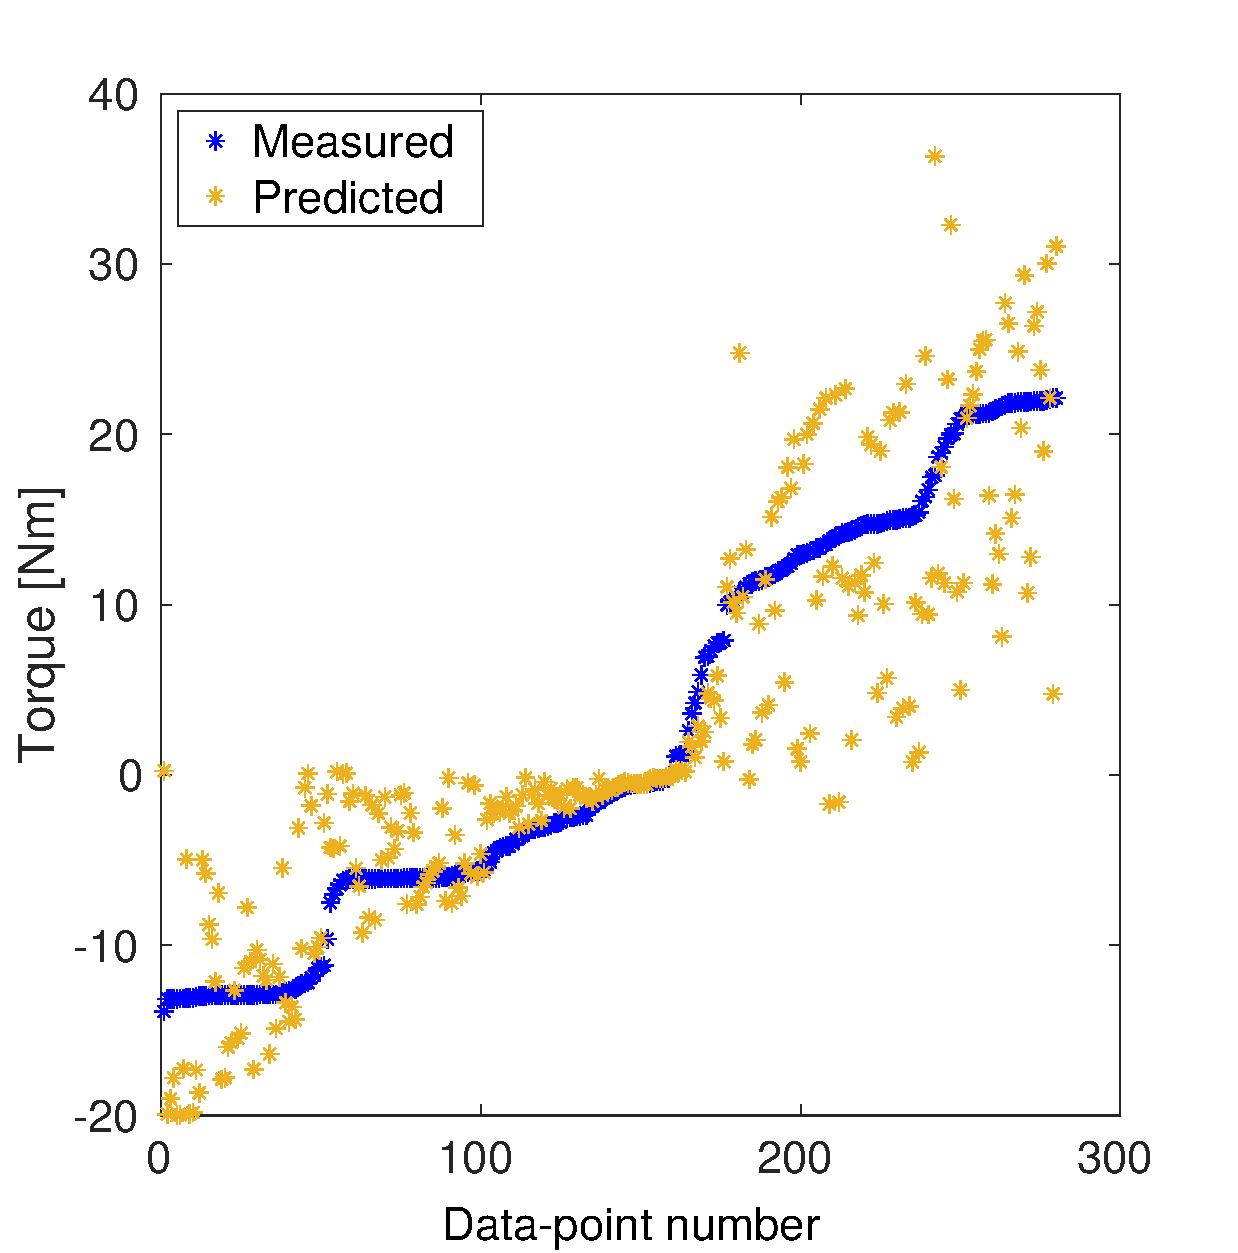
\includegraphics[width=\textwidth]{images/summer_school_study/measured_optimized_torque_B.pdf}%
    \caption{Measured values (blue) and values predicted by model B (orange).}%
    \label{fig:measured_optimized_torque_B}%
  \end{subfigure}%
  \caption{Resubstitution prediction: Measured and predicted torque values for the training data set. The measured points are ordered and numbered by magnitude, the order of the predicted points matches the order of the measured points.}%
  \label{fig:measured_optimized_torque}%
\end{figure}%

\subsection{Validation}\label{sec:res_validation}

The next evaluation uses the validation dataset and compares the predicted outputs of the models with the actual experimental values.
In contrast to the training data, where a small number $n$ of points was selected, we now use all captured values. This involves a total of \num{54e3} data points for a time span of $t=\SI{54}s$. 

\begin{figure}%
  \centering%
  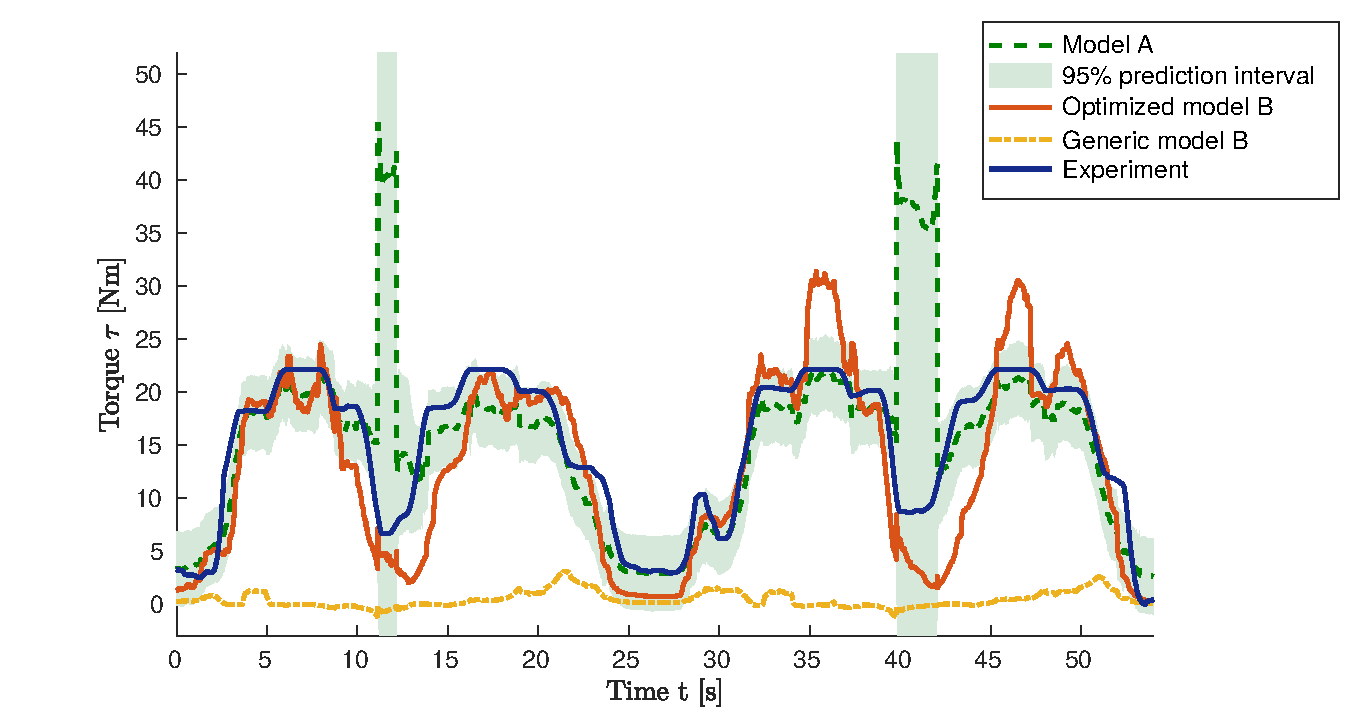
\includegraphics[width=\textwidth]{images/summer_school_study/validation_bv5_40_points.pdf}%
  \caption{Validation: Predicted torque values by model A (green), trained model B (red) and untrained model B (yellow), in comparison to the experimentally measured values (blue), for the validation data set.}%
  \label{fig:validation_bv5_40_points}%
\end{figure}%

The results are shown in \cref{fig:validation_bv5_40_points}. Comparing the green curve for model A with the blue curve for the experimental data, it can be seen that the predicted values match qualitatively for most of the time span. The predicted torque values appear consistently slightly smaller than the real values. Only for the two intervals $[\SI{11}s, \SI{12}s]$ and $[\SI{40}s, \SI{42}s]$ the predicted value is far off. The \SI{95}\percent{} confidence interval that was computed by the Gaussian Process spans a large range for these time intervals which implies that the model prediction is not to be trusted for this area. 

The biophysical model approach, model B, was tested in two variants. First, with the generic parameters from literature (yellow curve), second, with the subject-specific, optimized parameters (red curve). It can be seen that the generic model fails to predict the torque values whereas the trained model predicts reasonable values. These values are worse than most of the predictions from model A, but they succeed in giving a qualitative estimate about a low, medium or high torque output.

The match between model outputs $\tau_i$ and experimental data $\hat\tau_i$ can be quantified using the normalized root-mean-square error (NRMSE). This is a scaled version of the root-mean-square error (RMSE) and can be defined as
\begin{equation*}
  \begin{array}{lll}
    \text{RMSE} = \sqrt{\sum\limits_{i=1}^N (\tau_i - \hat{\tau_i})^2 / N},\\[4mm]
    \text{NRMSE} = \dfrac{\text{RMSE}}{\max\limits_i\{\hat\tau_i\} - \min\limits_i\{\hat\tau_i\}}.
  \end{array}
\end{equation*}
The NRMSE for model A is 0.267 which is worse than the value of 0.163 for the trained model B. The generic model B has the worst NRMSE of 0.547.

\subsection{Simplified Model A}\label{sec:res_simplified_a}
An advantage of model approach A is that it forgoes any biophysical description and the associated type of model error. It is a generic approach that does not require expert knowledge about the physiological structure. In the present study, however, some level of expert knowledge and physiological model was required in preprocessing the MoCap data, i.e. solving the inverse kinematics of the observed forearm movements to get the kinematic quantities of muscle lengths, velocities and moment arms. 

Since model A performed well in the previous validation study, we tested whether good results can also be achieved without this expert knowledge.
Consequently, the next study applies model approach A using only the elbow angle and no muscle lengths, velocities nor moment arms. Thus, the training data consists of input vectors $\bfx_i = (\phi_e(t_i), \gamma_B(t_i), \gamma_T(t_i))^\top \in \mathcal{X}$. In the following, this model is named \say{simplified model A} in contrast to the \say{full model A} that uses the complete set of input variables.

The results are shown in \cref{fig:measured_optimized_A2}. It can be seen that the resubstitution prediction in \cref{fig:measured_optimized_torque_A2} where the trained model is used to predict the training values shows a perfect fit. In contrast to the full model A, \cref{fig:measured_optimized_torque_A}, here, the learned input-output mapping shows no variance. However, the prediction for the validation dataset in \cref{fig:measured_optimized_torque_A3} shows a high error relative to the experimental data. The curve for the experimental data even lies outside the 95\% confidence interval of the prediction at some points. 

The simplified model A has a NRMSE value of 0.461. For comparison, the NRMSE values of the full and simplified model A and the generic and optimized model B are summarized in \cref{fig:nrmse}. 

This evaluation shows that simplified model A gives no useful results where the training input is too scarce. Instead, preprocessing of the measurements using a subject specific geometric model, as done for the full model A, is needed to allow for a useful prediction.

\begin{figure}%
  \centering%
  \begin{subfigure}[t]{0.48\textwidth}%
    \centering%
    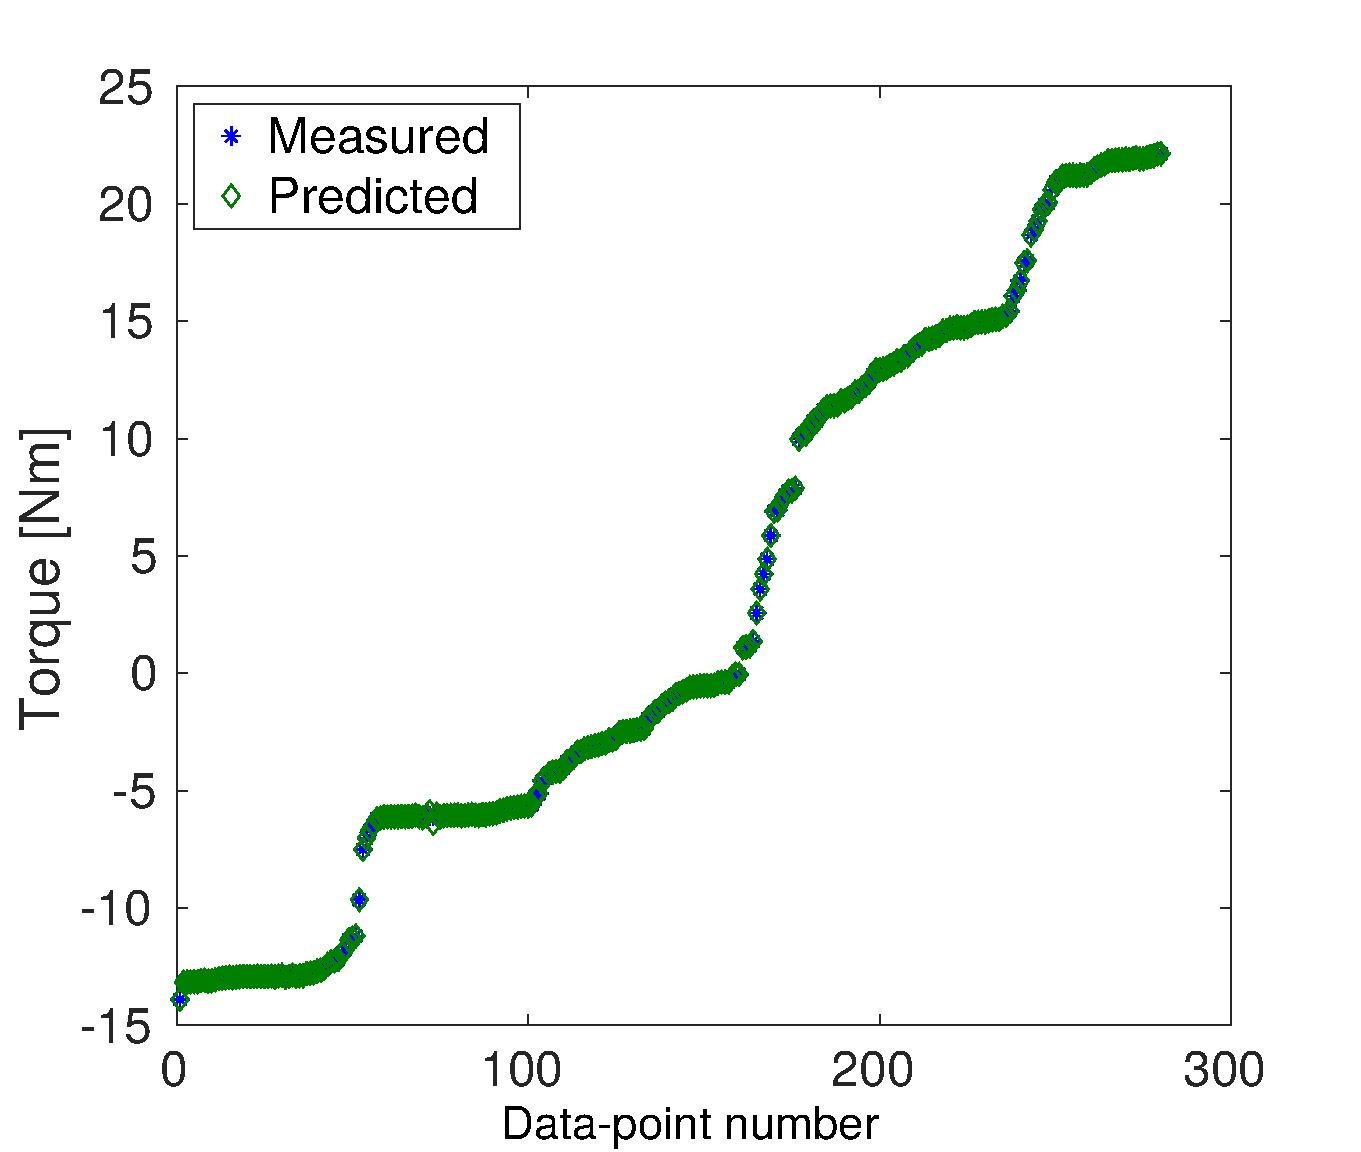
\includegraphics[width=\textwidth]{images/summer_school_study/measured_optimized_torque_A2.pdf}%
    \caption{Measured and predicted torque values of the training dataset, ordered and numbered by magnitude. The measured values (blue) and the values predicted by the Gaussian Process (green) lie on each other.}%
    \label{fig:measured_optimized_torque_A2}%
  \end{subfigure}%
  \quad
  \begin{subfigure}[t]{0.48\textwidth}%
    \centering%
    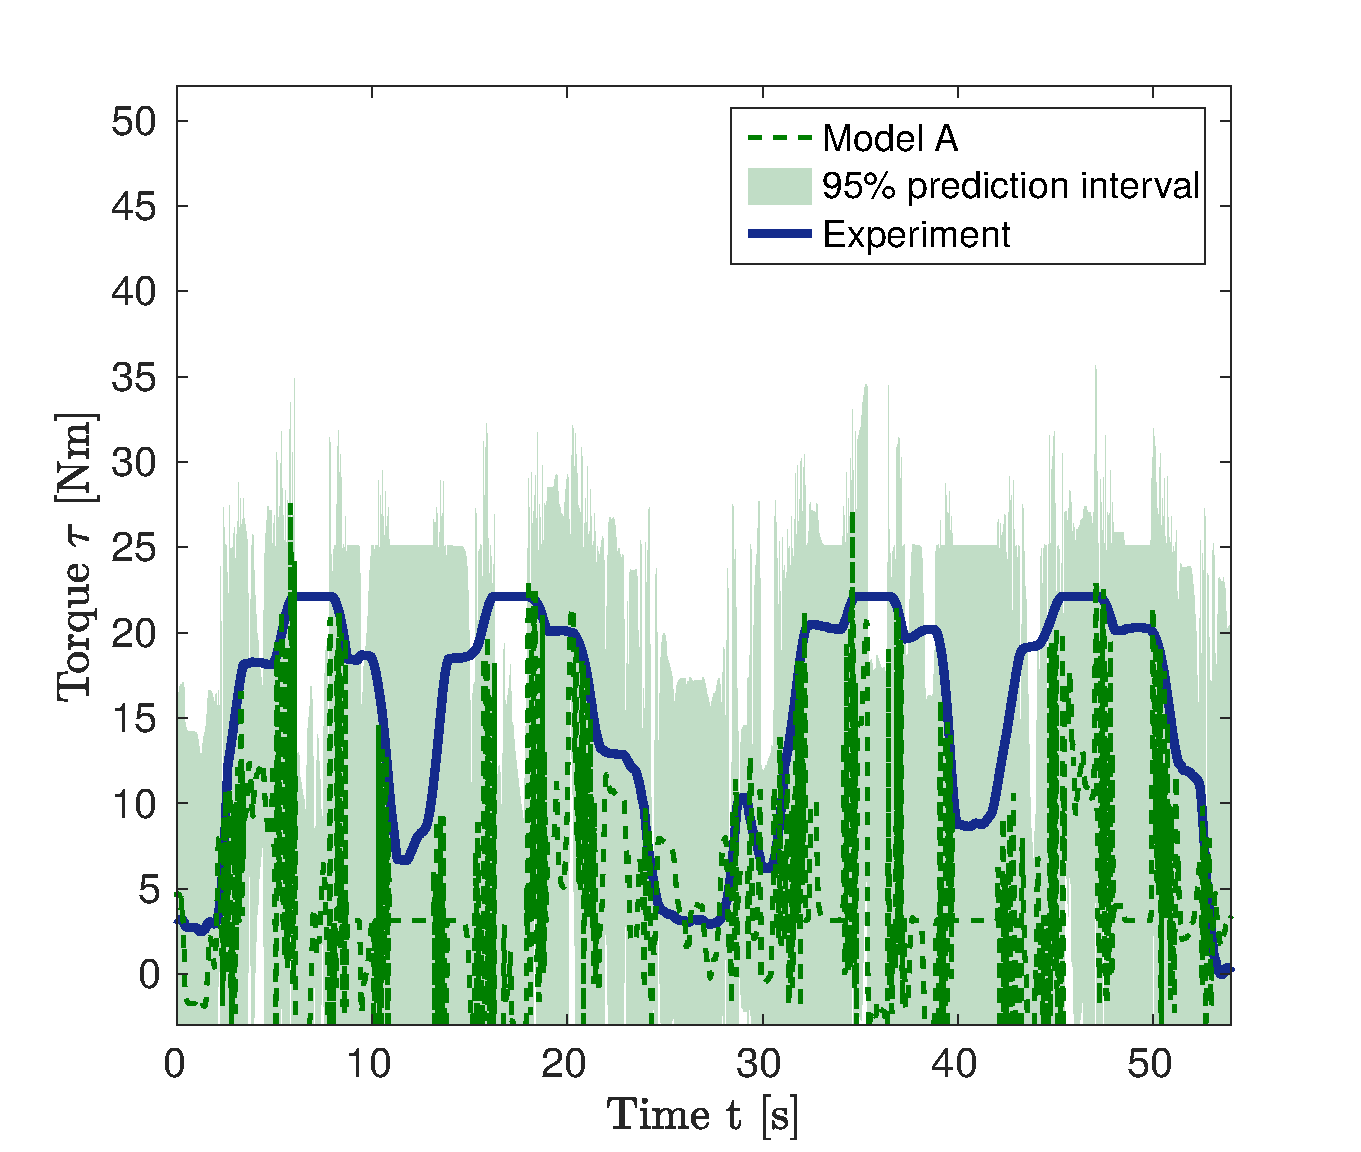
\includegraphics[width=\textwidth]{images/summer_school_study/validation_bv5_40_points_only_gamma_for_training.pdf}%
    \caption{Predicted torque values for the validation trials (green dotted line), 95\% confidence interval (light green) and the reference values of the experiment (blue). The plot reveals bad prediction capabilities of the simplified model A.}%
    \label{fig:measured_optimized_torque_A3}%
  \end{subfigure}%
  \caption{Result for the simplified model A, where, apart from the free calcium ion contractions, only the elbow angles, $\phi_e$, are used as training input instead of MTU lengths, velocities and moment arms.}
  \label{fig:measured_optimized_A2}%
\end{figure}%

\subsection{Insights of Model B}\label{ref:res_insights_b}
An advantage of model approach B is that the trained parameters are physically meaningful and allow insight into the properties of the subject specific model. Furthermore, the quality of the training data can be assessed. \Cref{fig:biceps_working_area} shows the force-length relation of the biceps muscle model using the generic and the optimized parameter values. It can be seen that the subject-specific model has a smaller slope of the force curve. 
All points of the training data set are indicated by red crosses on the curves and show the operating range of the muscle in which the model has been trained. It can be seen that the experimental training data are limited to a small range of the muscle length below its optimal CE length $l_{\CE,\text{opt}}$. In order to improve the quality of the model predictions for this subject, specific additional experimental trials can be designed for model training. They can be designed to fill in values in the missing range of operation, which in this case is for larger muscle extensions.

A low computational time of the offline parameter identification and the online evaluation of the two models would be an important measure for their practical applicability. In the present study, the training phase of Model A, i.e., optimization of the quantities for the Gaussian Process Regression using 280 training data points took \SI{2.24}{\second}. The evaluation of Model A for the validation data set containing \num{54e3} points had a duration of \SI{116}{\milli\second}.

The runtimes for model B were significantly higher. The parameter optimization lasted \SI{25}{\minute} \SI{16}{\second} and the evaluation for the validation data set had a duration of \SI{13}{\second}.

The large differences in runtime between models A and B can be explained by the inefficient implementation of the biophysical model using the MATLAB programming language. During parameter identification, this model needs to be evaluated iteratively in the optimization algorithm. In contrast, the optimization within model A works with an internal implementation of the Gaussian Process which was optimized during development of the particular MATLAB functionality.
In general, the evaluation of Gaussian Process Regression has cubic time complexity whereas, for the parameter optimization of model B, iterative solvers with linear time complexity exist.

\begin{figure}%
  \centering%
  \begin{subfigure}[t]{0.47\textwidth}%
    \centering%
    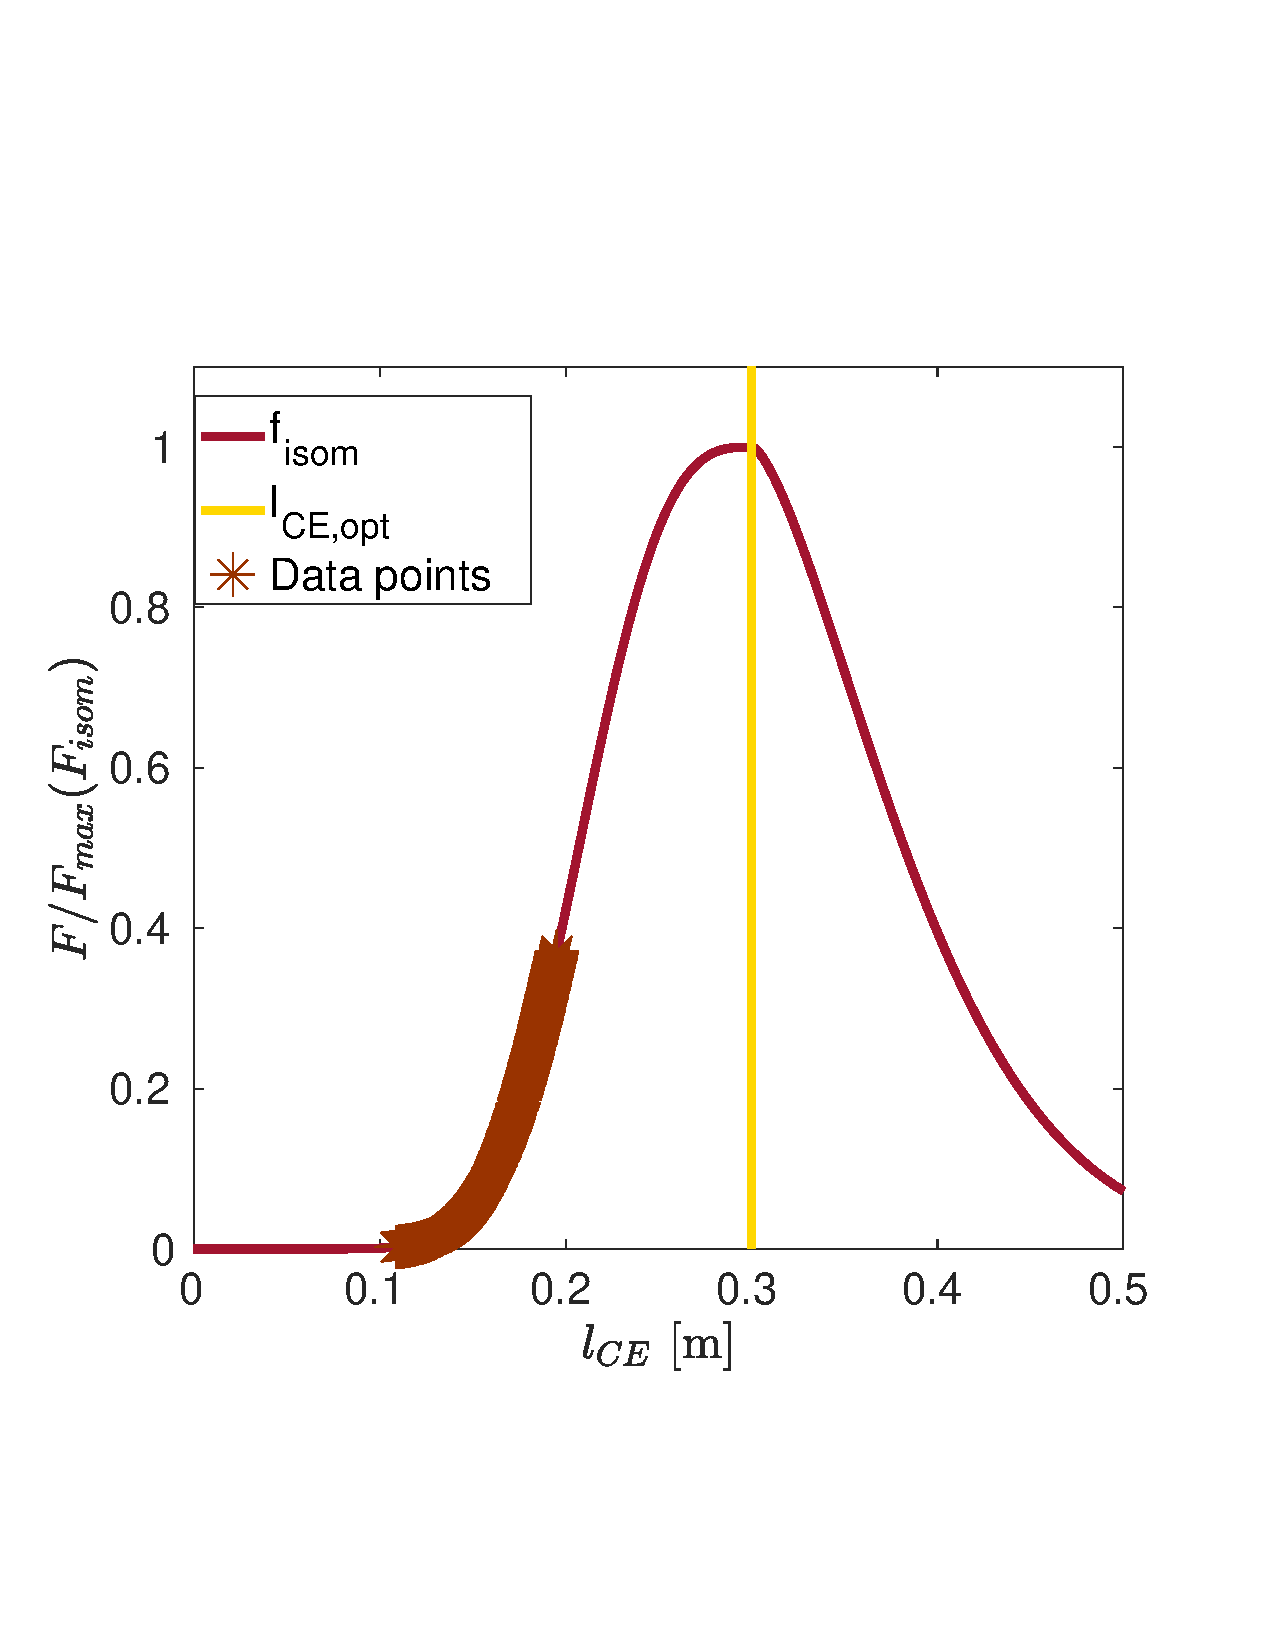
\includegraphics[width=\textwidth]{images/summer_school_study/biceps_initial.pdf}%
    \caption{Model with generic parametrization.}%
    \label{fig:biceps_a}%
  \end{subfigure}%
  \quad
  \begin{subfigure}[t]{0.47\textwidth}%
    \centering%
    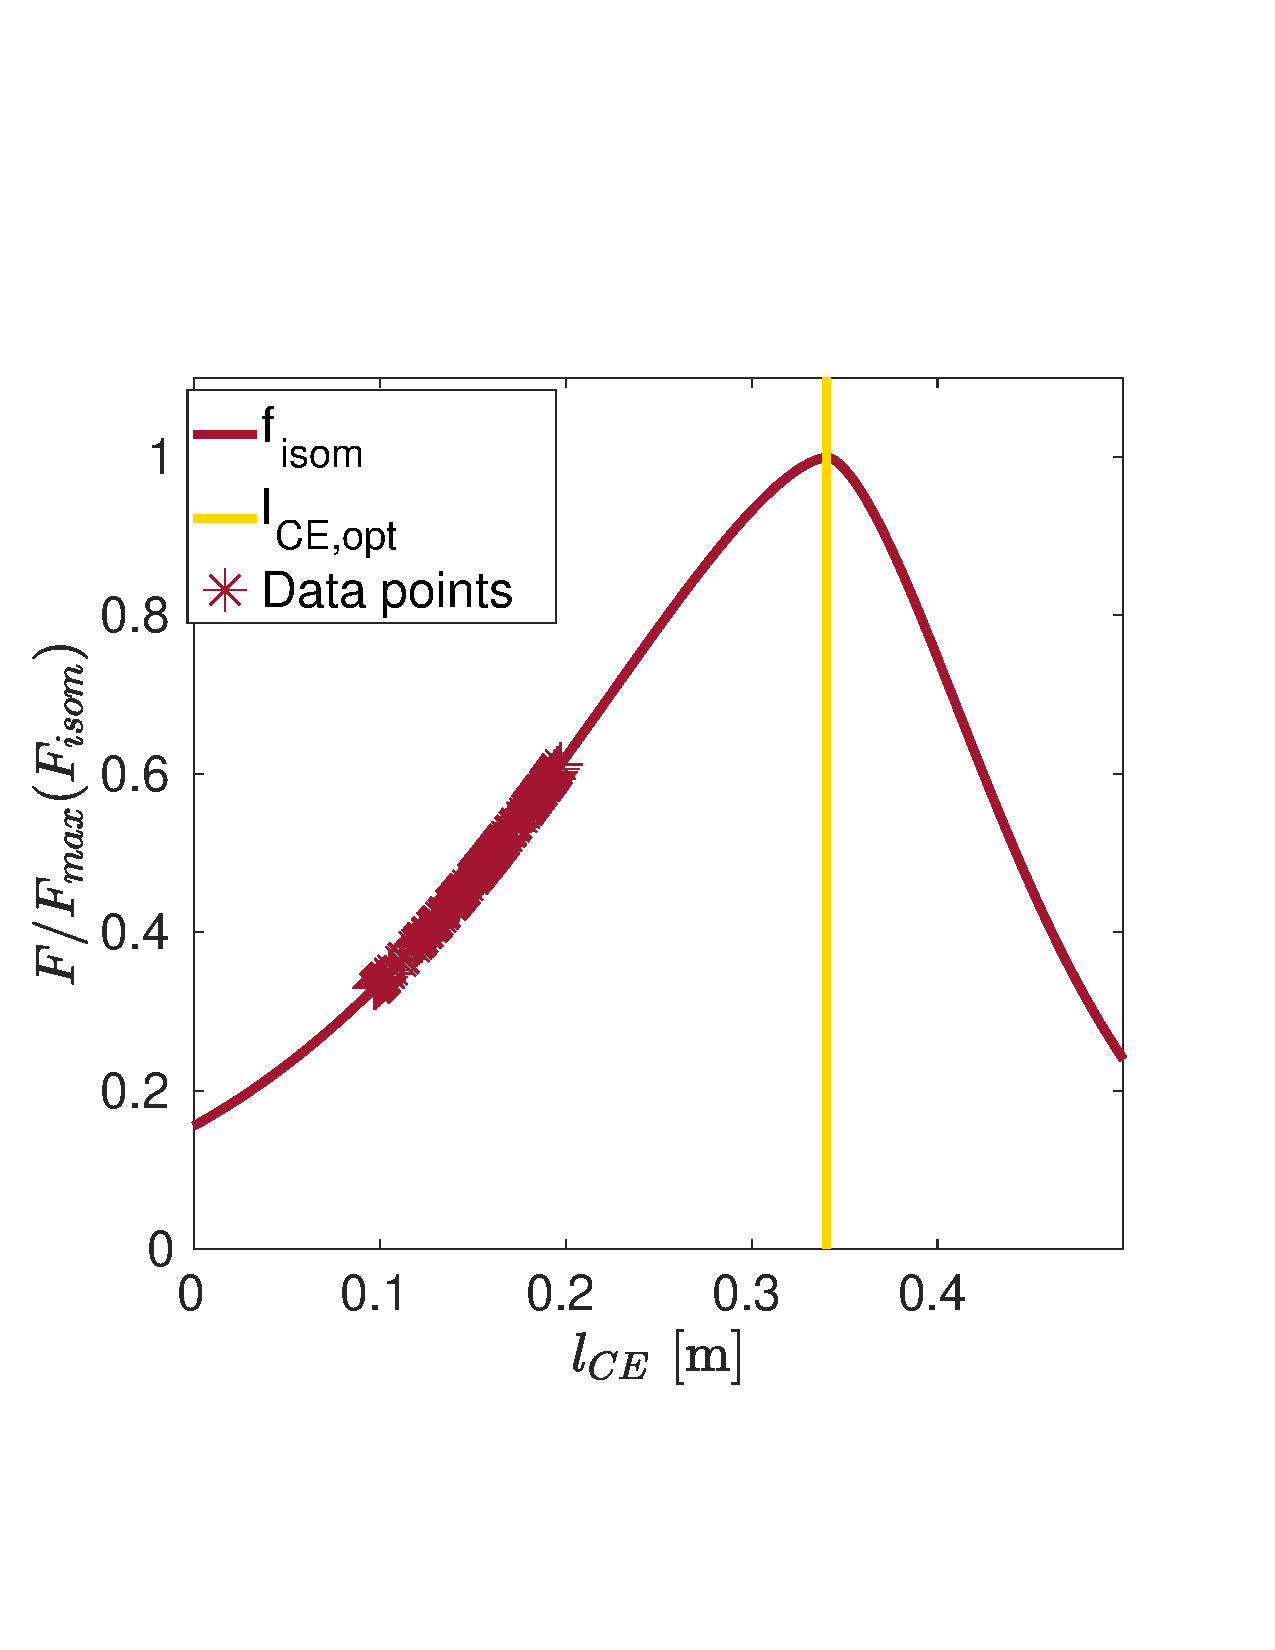
\includegraphics[width=\textwidth]{images/summer_school_study/biceps_optimized.pdf}%
    \caption{Model with subject-specific parametrization.}%
    \label{fig:biceps_b}%
  \end{subfigure}%
  \caption{Isometric force-length relation of the CE for the biceps model, analogue to \cref{fig:force_curves_generic_length}, but additionally with training data points. The points are placed on the model curve and visualize the predicted relative forces for the lengths of the CE that occurred during the training trials.}%
  \label{fig:biceps_working_area}%
\end{figure}%


\begin{figure}%
  \centering%
  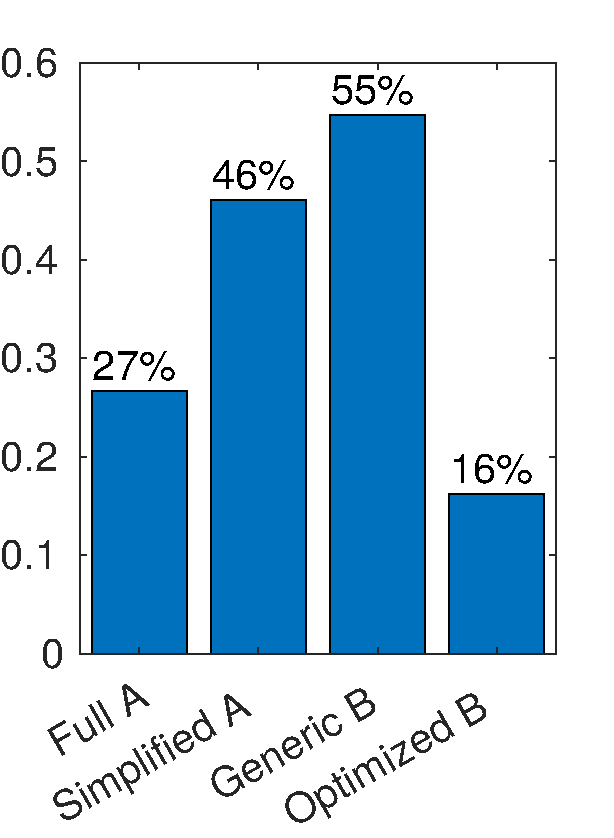
\includegraphics[width=0.35\textwidth]{images/summer_school_study/nrmse.pdf}%
  \caption{Normalized Root Mean Square errors (NRMSE) of the validation trials between the respective models and the measured values. A lower error value means a better fit.}%
  \label{fig:nrmse}%
\end{figure}%

\section{Conclusion}\label{sec:study_conclusion}
In this study, elbow torques during flexion and extension of the upper arm were predicted from motion capture data and EMG measurements. Two models, A and B, were developed. Model A is non-parametric and uses Gaussian Process Regression. Model B is biophysically informed and involves two state-of-the-art Hill-type muscle models for biceps and triceps. Experiments were conducted to generate training and validation data. These training data were used for model parameter identification. Predictions from the two models were compared to real experimental values using the validation data.

Regarding the formulation and implementation, model A requires low effort and no special knowledge about the model, except where experimental motion data is preprocessed for a specific subject. In contrast, model B needs expert knowledge about the biophysical structure and the implementation of all comprised models.

Similar holds for the offline training phase. There are no parameters in model A that have to be tuned manually, which allows a quick start. Conversely, model B requires the appropriate definition of initial values and physiological constraints for the optimization problem. However, this can also be seen as an advantage for model B, as a-priori knowledge can be integrated in such a model.

On the other hand, an advantage of model A is that additional experimental data, e.g., from neighboring muscles or additional sensors, can easily be added to the model. This is not possible with model B, where the model formulation would have to be changed.

Our studies showed that both models were able to predict the levels of torque reasonably. 
\Cref{fig:nrmse} showed the best score for model A, followed by model B. It was also seen that the generic parametrization of model B does not yield a useful prediction. The same is true for a simplified version of model A, where the elbow torque was used as training input instead of derived quantities from the motion capture system that required a complex preprocessing step.

Both models provide possibilities to assess the confidence of their predictions. With model A, confidence intervals can be computed directly from the Gaussian Processes. Their usefulness was shown in the validation where regions with large errors also had a large confidence interval. 
Model B allows insight into force-length and force-velocity characteristics of the two involved muscles. The operating ranges of the muscles during the experiments can be visualized and allow assessing whether the desired model features were covered by the training phase and, thus, will yield a good prediction.

In our study, runtimes were low for model A and high for model B in both offline and online phases. However, this is due to our prototypical implementation of model B. For larger data sizes and a more sophisticated implementation, the reverse effect is expected. The runtime complexity for the training phase is better for model B (linear in time) compared to model A (cubic in time). For the online phase, costly integration over data points is needed for model A whereas model B directly provides a differential equation of the system that can be solved efficiently. 

If EMG is used to control an exoskeleton that supports the movement of the limb, it is known that the measured signals are ahead of the intended movement by a small offset. This is a result of the time delay in the neuromusculoskeletal system. This property gives the assistive exoskeleton a short time to predict the intended movement and thereby allows a seamless integration of the artificial device with human control.

When targeted at such a real-time application, both models could be considered to be integrated into the control. Model A better fits the use case of a device that could be (re\nobreakdash-)calibrated by the patient itself. Because of the built-in estimation of prediction quality, compliance and safety could be ensured more easily even for imperfect training.
Model B would need a controlled environment such as a specialist's laboratory and careful assistance for the calibration process.
After calibration, it would promise a more natural and more responsive experience because of the subject-specific model and possibly smaller compute times.

Where real-time application is not a requirement, biophysically informed models have a high potential to leverage the understanding how the human neuromusculoskeletal system operates for given tasks.
In model B of this study, the kinematics and individual muscle dynamics were described close to the current  understanding of the system. However, several aspects where not modeled as detailed as possible. The pathway from neural stimulation to excitation and activation of the muscle, the recruitment strategies including different motor units, neural feedback loops as well as effects stemming from the 3D geometry of the muscle were not considered. Therefore, this thesis develops a more detailed, biophysically informed model including these properties in the following chapters.

The presented study reproduced what similar studies in literature have shown: Subject-specific model identification for Hill-based torque prediction models can vastly improve the prediction quality compared to generic models. Our work adds to the common knowledge that this holds also for the four-element Hill-type model that was used for model B. Furthermore, a comparison with Gaussian Process Regression was given, various advantages and disadvantages of these two approaches were identified. Future work can test the two models with more subjects and increase the variety of motion in the training experiments. For example, effects resulting from high contraction velocities or eccentric contractions could be investigated to evaluate the model's potential in more complex movements.
